\section{Simulation}

Das folgende Kapitel beinhalten die Auswertungen der Simulationen, die mit den Tools Plecs und Matlab durchgeführt wurden. Im ersten Teil des Kapitels, simulierte man mit Matlab die zwei bekannten Steuerungsarten, Phasenanschnitt- und Schwingungspaketsteuerung, des einphasigen Steuersignal. Im zweiten Teil führte man die gleichen Verfahren mit Plecs durch. Anschliessend verglich man die Resultate der beiden Simulationen miteinander und konnte so die Richtigkeit der Überlegung und der Modulation bestätigen. Aufgrund dessen konnte mit Plec, das dreiphasige Steuerverfahren und eine Kombination der beiden Systeme im ein- und dreiphasigen System simuliert werden. 



\subsection{Simulation mit Matlab}
Um die einphasige Plecs-Simulationen der Phasenanschnitt- und Schwingungspaketsteuerung zu verifizieren wurde parallel zur Plecs-Simulation das gleiche Verfahren mit Matlab vorgenommen. Mit Hilfe dieser Überprüfung konnte davon ausgegangen werden, dass die die Überlegungen sowie der Aufbau der Plec-Simulation stimmt und somit ohne weiteres bedenken das dreiphasige Vorgehen der zwei Verfahren mit Plecs verwirklichen kann. Im folgenden Abschnitt wird nun aufgezeigt, welche Überlegungen man bei den Matlabfunktionen vorgenommen hat und wie die Ergebnisse zustande kamen.

Die ersten Funktionen, die man simulierte, waren periodische Sinusfunktionen im Zeitbereich mit verschiedenen Phasenanschnitten. Die Periodenlänge definierte man dabei auf 2$\pi$ und die Amplitude des Sinus auf ± 1. Der Winkel des Phasenanschnittes wurde mit verschieden, geläufigen Werte wie zum Beispiel $30^\circ$, $45^\circ$, $60^\circ$, $90^\circ$ oder $120^\circ$ betrachtet. In den Abbildungen \ref{fig:Einganssignal 60} erkennt man die Sinusfunktionen mit einem Phasenanschnitt von links \ref{fig:Einganssignal 60} $60^\circ$ und rechts \ref{fig:Einganssignal 90} $90^\circ$. Weitere Funktionen mit den anderen Winkeln sind im Anhang ersichtlich.
 

\begin{figure}[h]
	\centering
	\subfloat[][]{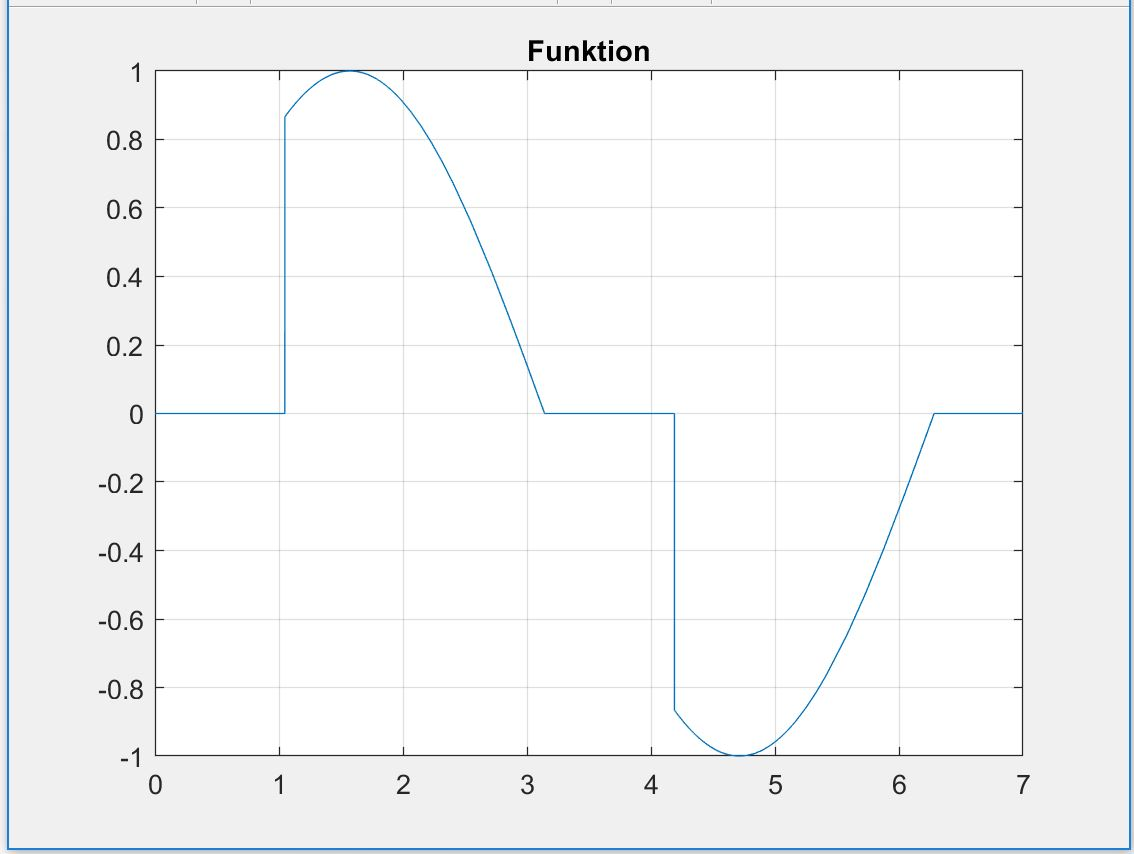
\includegraphics[width=0.47\linewidth]{eingangssignal_60.png}\label{fig:Einganssignal 60}}\qquad
	\subfloat[][]{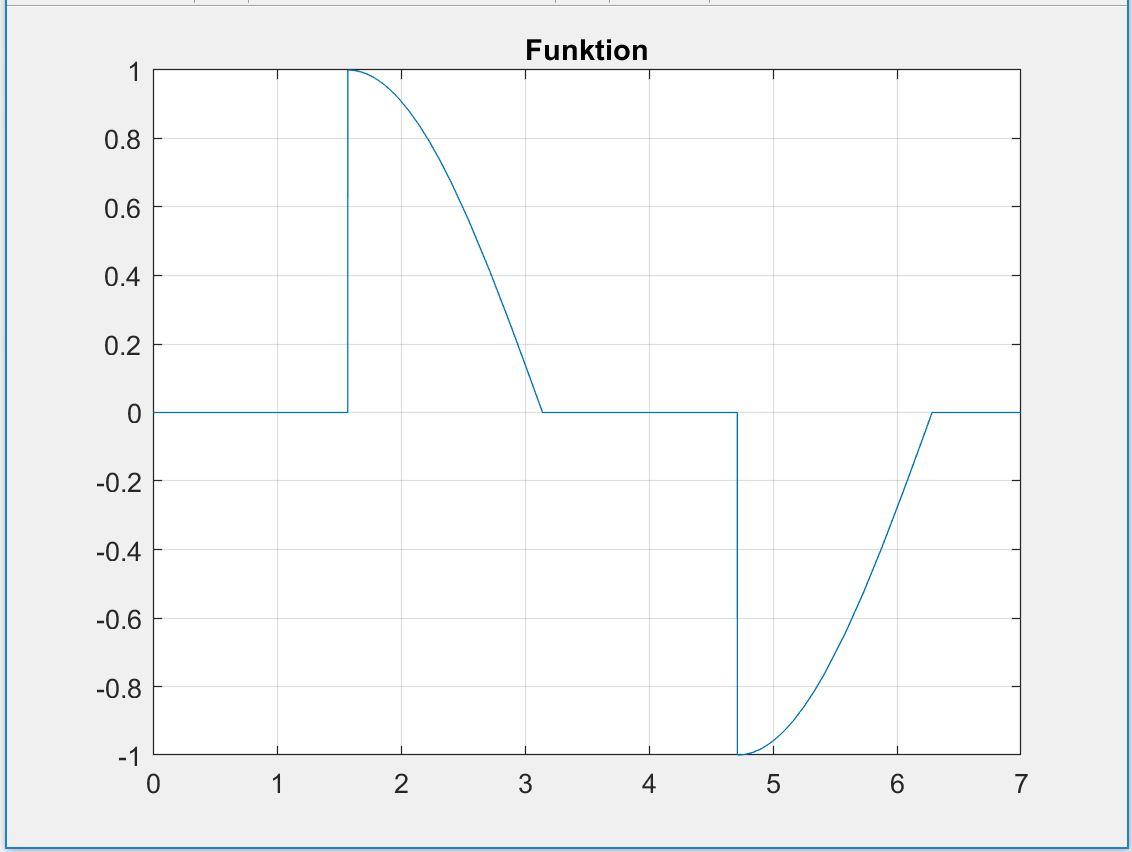
\includegraphics[width=0.47\linewidth]{eingangssignal_90.png}\label{fig:Einganssignal 90}}
	\caption{Einganssignal mit Phasenanschnitt (a) $60^\circ$ (b) $90^\circ$}
	\label{fig:eingangssignal_mit_Matlab}
\end{figure} 


Als nächstes nahm man die Zerlegung der Funktion in verschiedene Frequenzanteile vor. Dies wird auch als Fourier-Analyse bezeichnet. Man berechnete zuerst die Fourier-Koeffizienten $a\textsubscript{0}$, $b\textsubscript{n}$ und $a\textsubscript{n}$ und konnte danach mit den folgenden Formeln das Amplituden- und Phasenspektrum berechnen.



 Die Darstellung im Zeitbereich beziehungsweise im Frequenzbereich sind äquivalent, sie enthalten also die vollständige Information über die Funktionen. Im Spektrum benutzt man die vertikalen Linien, um die Frequenzkomponenten anzugeben. Die x-Achse ist somit die Frequenz der Frequenzkomponente und die y-Achse zeigt die Länge der Amplitude an. In den untenstehenden Grafiken \ref{fig:Amplituden- und Phasenspektrum} erkennt man das Amplituden- und Phasenspektrum des in Abbildung \ref{fig:eingangssignal_mit_Matlab} dargestellten Signale.

\begin{figure}[h]
	\centering
	\subfloat[][]{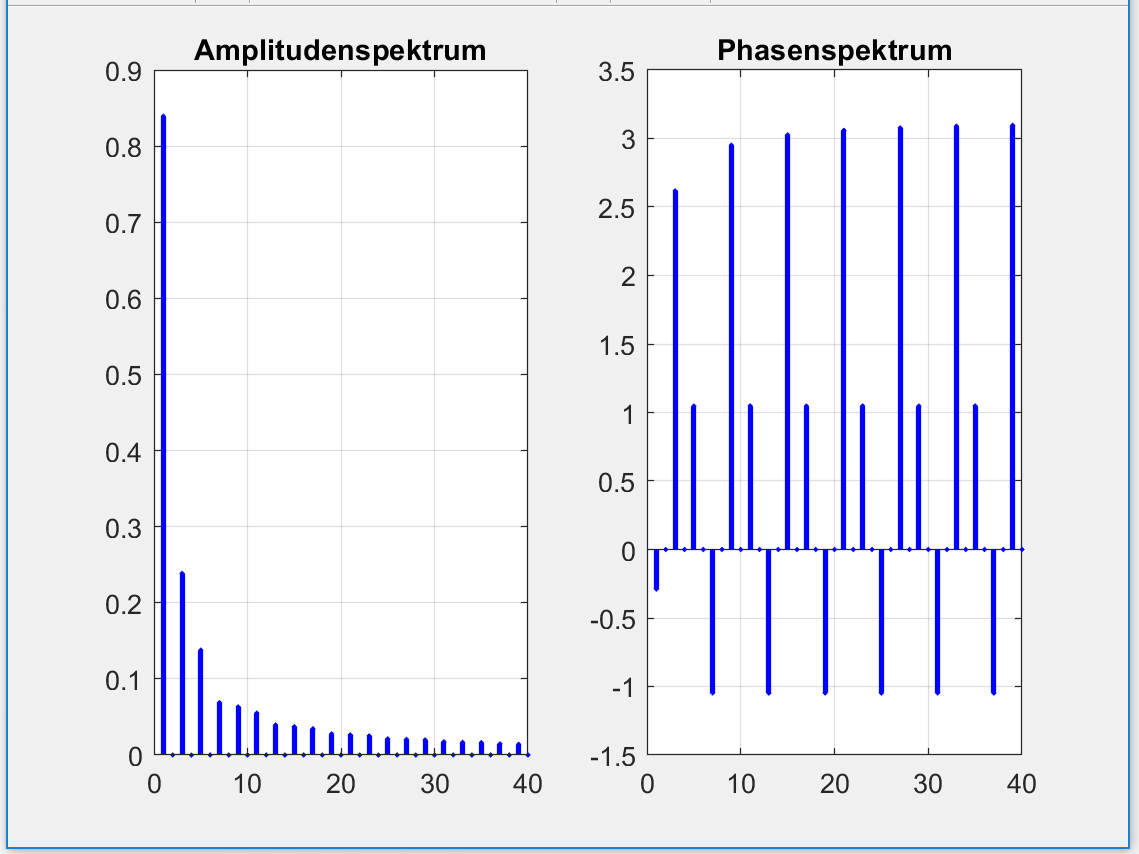
\includegraphics[width=0.47\linewidth]{A_PH_60.png}\label{fig:Amplituden- und Phasenspektrum 60}}\qquad
	\subfloat[][]{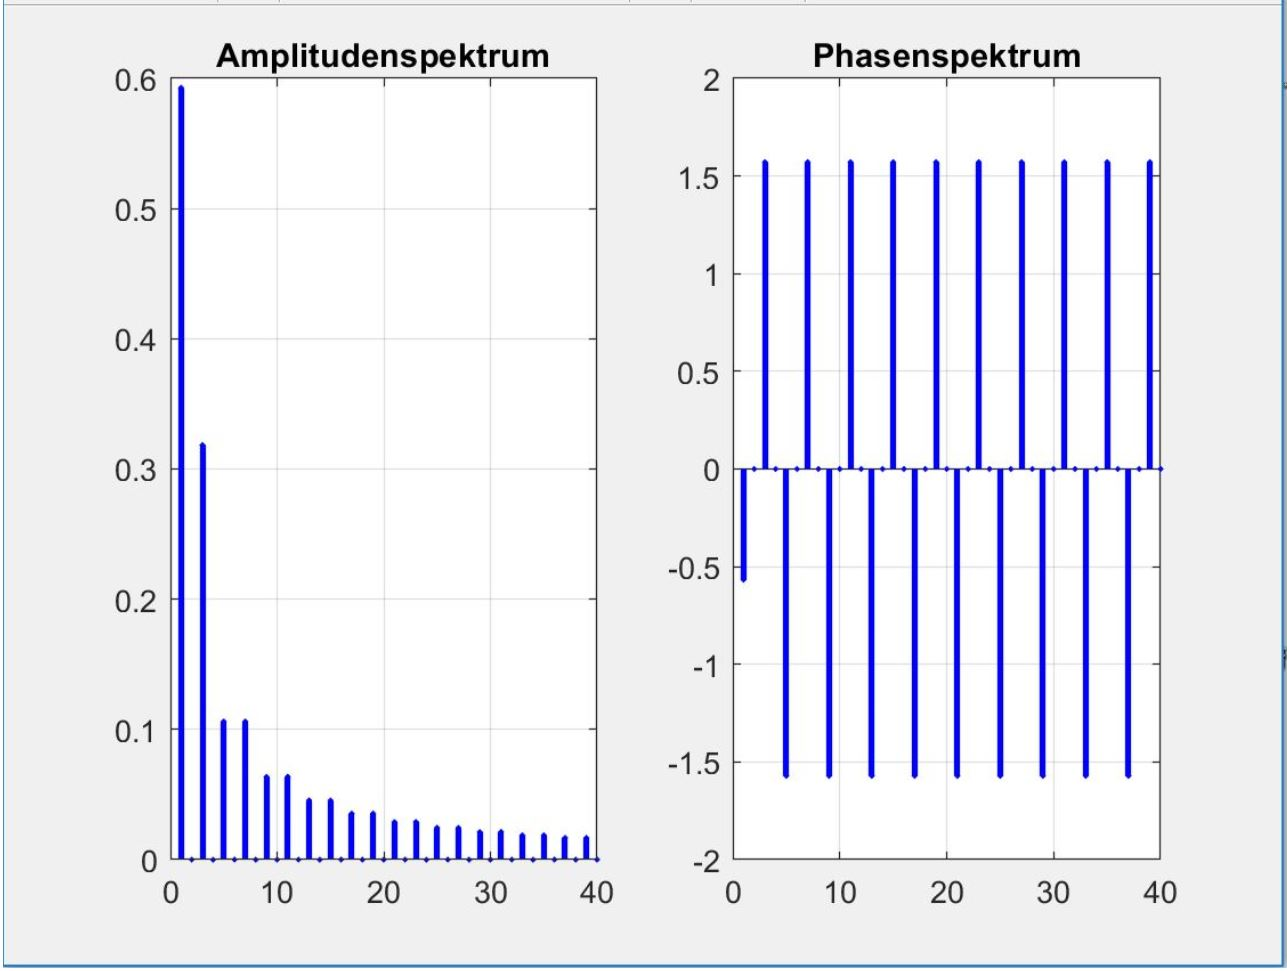
\includegraphics[width=0.47\linewidth]{A_PH_90.png}\label{fig:Amplituden- und Phasenspektrum 90}}
	\caption{Amplituden- und Phasenspektrum (a) $60^\circ$ (b) $90^\circ$}
	\label{fig:Amplituden- und Phasenspektrum}
\end{figure} 

Zur Überprüfung der Berechnungen und der Darstellung des Amplituden- und Phasenspektrum, wurde mit diesen zwei Spektren das Eingangssignal rekonstruierte. Die Signale erkennt man auf der nächsten Abbildung \ref{fig:Rekonstruiertes Signal}. Es ist ersichtlich das die Rundung des Sinus nicht genau dem, des eigentlichen Signal entsprechen \ref{fig:eingangssignal_mit_Matlab}. Dies kommt davon, dass man die Funktion in «nur» 40 Frequenzanteile unterteilt hat. Würde man eine grössere Anzahl Anteile verwenden, so könnte das Rauschen verkleinert werden. Da man jedoch nur einen ungefähren Vergleich der beiden Funktionen haben möchte, reicht diese Anzahl völlig aus. 

\begin{figure}[h]
	\centering
	\subfloat[][]{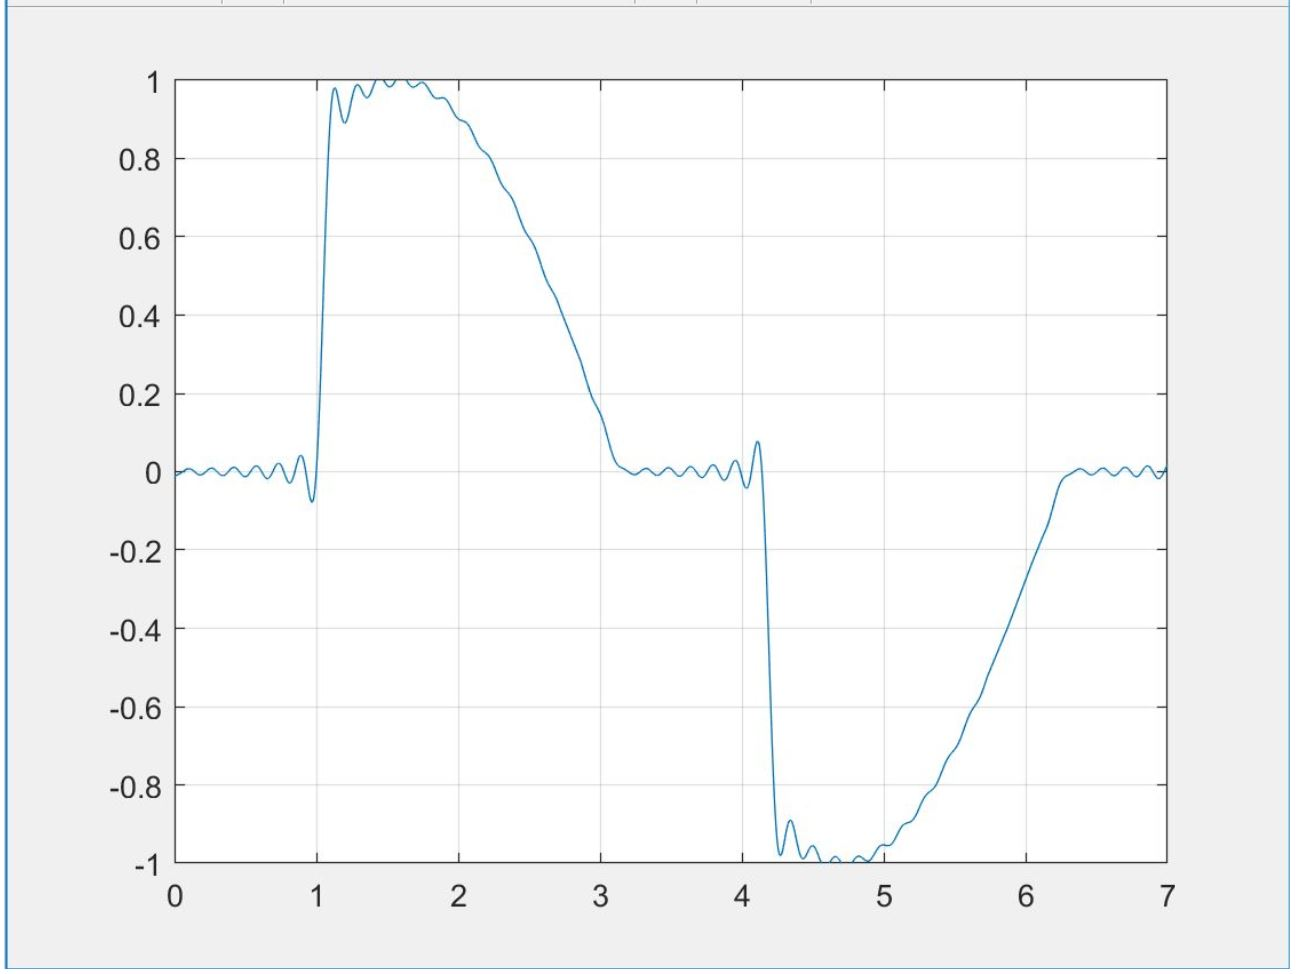
\includegraphics[width=0.47\linewidth]{re_eingangssignal_60.png}\label{fig:rekonstruiertes Signal 60}}\qquad
	\subfloat[][]{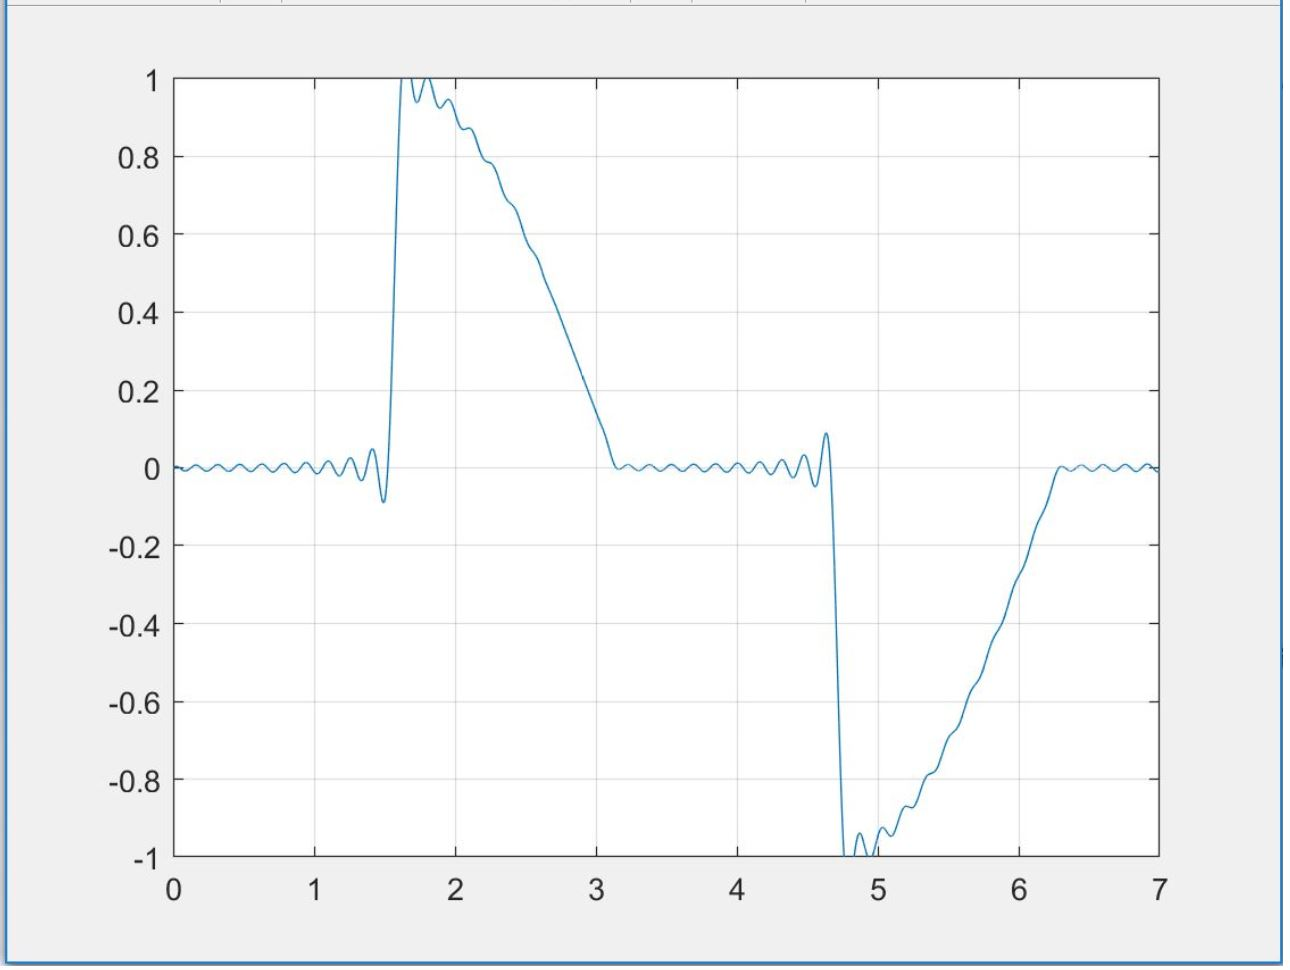
\includegraphics[width=0.47\linewidth]{re_einganssignal_90.png}\label{fig:rekonstruiertes Signal 90}}
	\caption{Rekonstruiertes Signal (a) $60^\circ$ (b) $90^\circ$}
	\label{fig:Rekonstruiertes Signal}
\end{figure} 


Nach dem man das Phasenanschnittsignal, das Amplitudenspektrum,  das Phasenspektrum und das rekonstruierende Eingangssignal von Hand berechnet und geplottet hat, überprüfte man mit Hilfe der FFT-Funktion (Fast Fourier Transform) von Matlab die Werte und die Grafiken. In der folgenden Abbildung \ref{fig:FFT mit Matlab} erkennt man die Plots bei einem Winkel von $60^\circ$. Bei dem Amplituden- und Phasenspektrum wurde die x-Achse so normiert, dass die Werte ein Vielfaches der Grundfrequenz von 50 Hz sind. So ist zum Beispiel der Wert bei 500 beim FTT zu vergleichen mit dem Wert 10 bei den Spektren die von Hand berechnet wurde.

\begin{figure}[ht!]
	\centering
	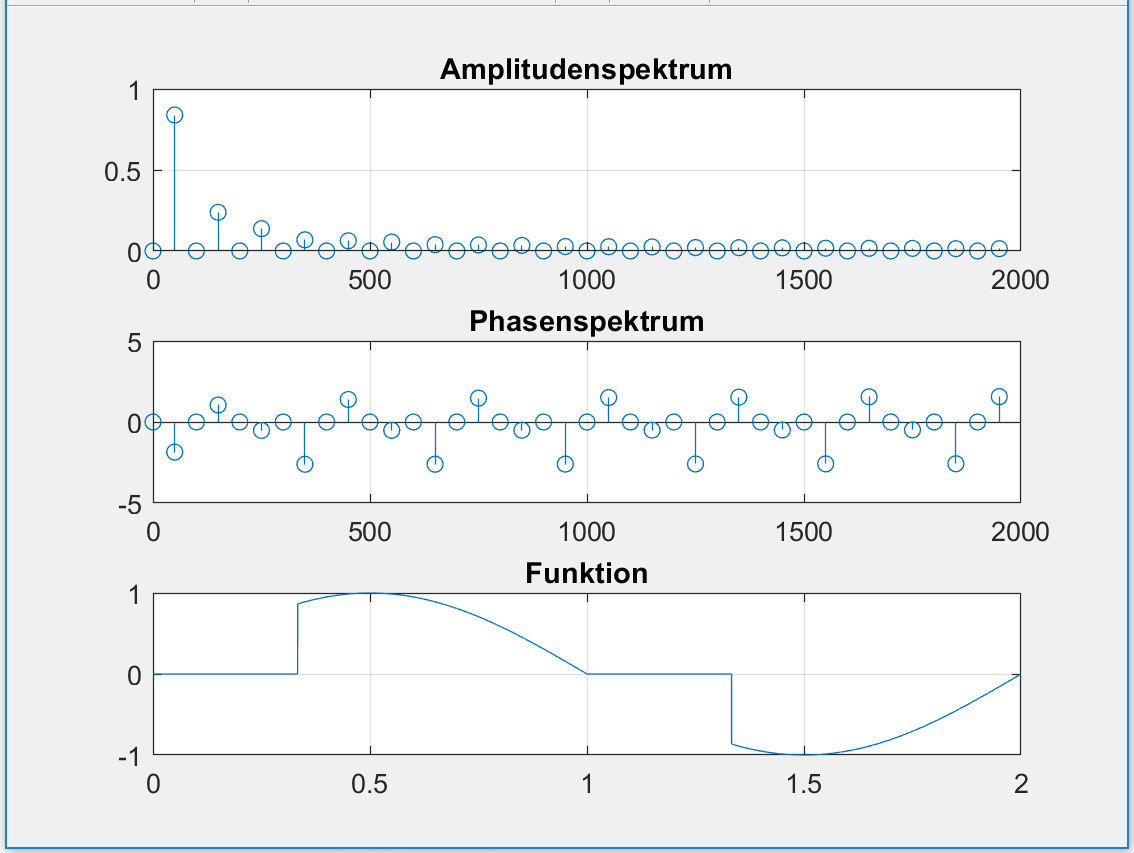
\includegraphics[scale=0.7]{FFT_mit_Matlab.png}	
	\caption{FFT mit Hilfe der Matlabfunktion}
	\label{fig:FFT mit Matlab}
\end{figure}

Bei der zweiten Funktion, die zu überprüfen und simulieren war, handelte es sich um eine Schwingungspaketsteuerungen. Die komplette Paketdauer beträgt bei den abgebildeten Funktionen 20 Halbwellen \ref{fig:Schwingungspaket Matlab}. Es wurden nun verschiedene Einschaltverfahren untersucht. In der Grafik  erkennt man links \ref{fig:Schwingungspacket 0.5} einen duty cycle von 0.5, es sind dementsprechend immer 10 Halbwellen  ausgeschaltet und die anderen 10 eingeschaltet. Auf der rechten Seite \ref{fig:Schwingungspacket 0.8} beträgt der Wert des duty cycle 0.8. Es sind also zuerst 4 Halbwellen ausgeschaltet und die restlichen 16 Halbwellen werden angesteuert. Für einen sinnvollen Vergleich mit der Plec-Simulation untersuchte man 5 Schwingungspakete. Die Leistungen der rechten Funktion ist somit 1/2 und die der linken 8/10 so gross wie die der normalen Netzspannung.

\begin{figure}[ht!]
	\centering
	\subfloat[][]{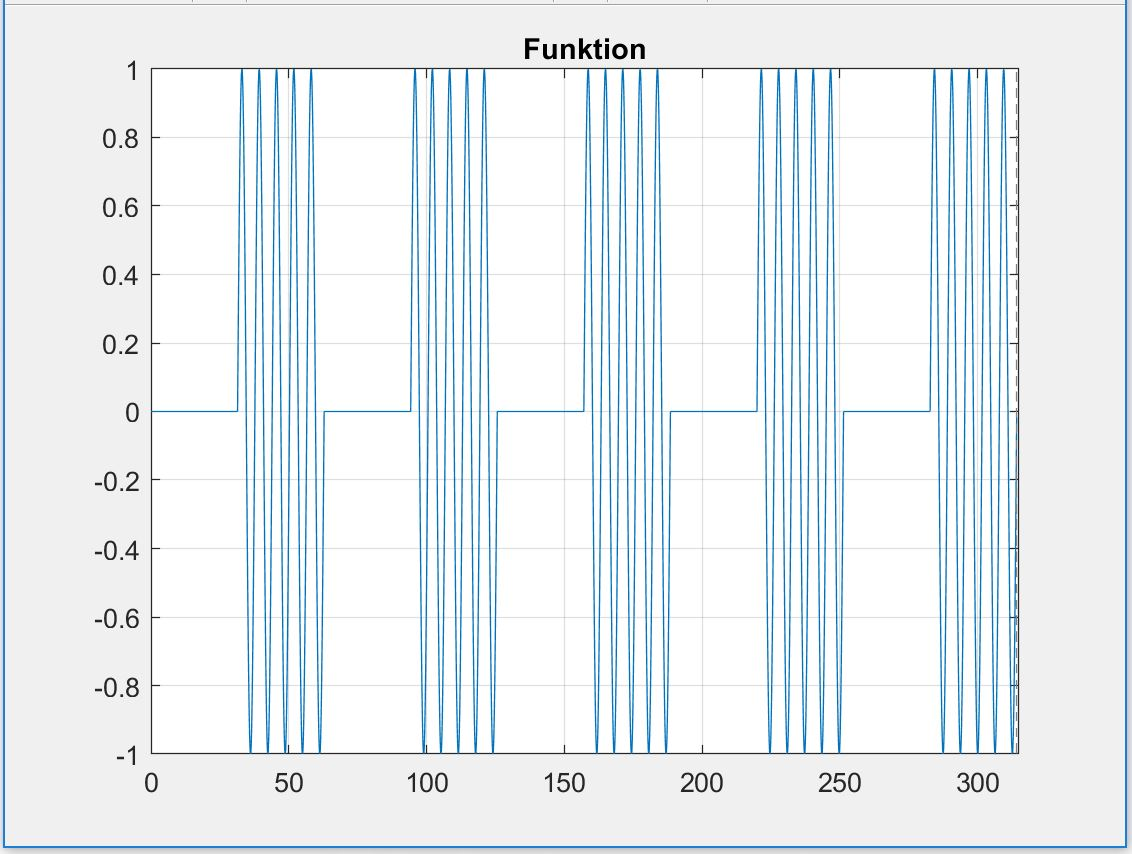
\includegraphics[width=0.45\linewidth]{Schwingungspaket_0_5.png}\label{fig:Schwingungspacket 0.5}}\qquad
	\subfloat[][]{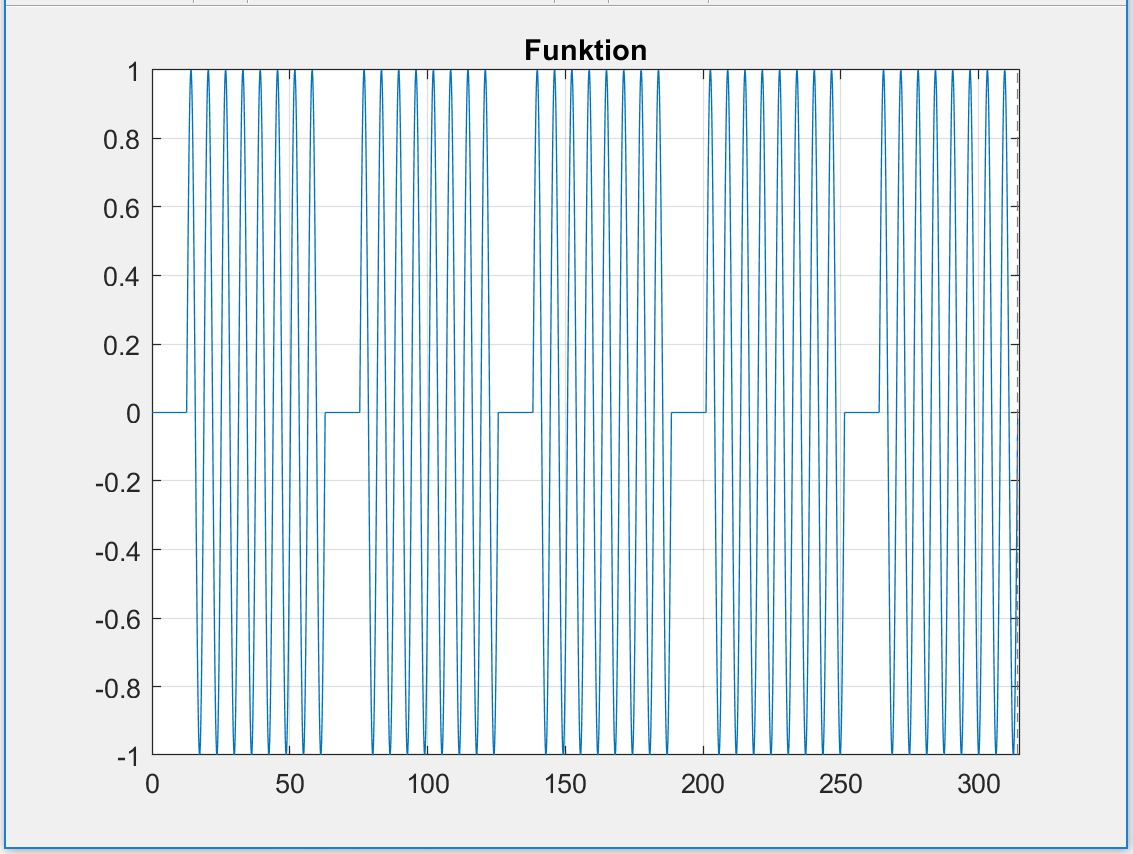
\includegraphics[width=0.45\linewidth]{Schwingungspaket_0_8.png}\label{fig:Schwingungspacket 0.8}}
	\caption{Schwingungspaket mit einem duty cycle von (a) 0.5 (b) 0.8}
	\label{fig:Schwingungspaket Matlab}
\end{figure} 

Um auch hier die Plecs-Simulation zu überprüfen, stellte man das absolute lineare Spektrum dar \ref{fig:Schwingungspaketspektrum Matlab}. Die unteren  Abbildungen zeigen die Spektren, links mit einem duty cycle von 0.5 \ref{fig:Schwingungspacketspektrum 0.5} und rechts mit einem von 0.8 \ref{fig:Schwingungspacketspektrum 0.8}. Interessant sind da vor allem die Subharmonischen Schwingungen, welche sich unterhalb der Grundfrequenz von 50 Hz befinden. Sie sind jeweils auf der linken Seite der Grafiken veranschaulicht. Damit man einen besseren Überblick über die Oberschwingungen erhält, wurde das Spektrum bis auf 1000 Hz erweitert. Dies ist auf der rechten Seite des jeweiligen Bildes ersichtlich. Vergleicht man die zwei Bilder erkennt man, dass je höher der duty cycle ist, desto höher ist der Peak-Wert bei der Grundfrequenz von 50 Hz. 

\begin{figure}[ht!]
	\centering
	\subfloat[][]{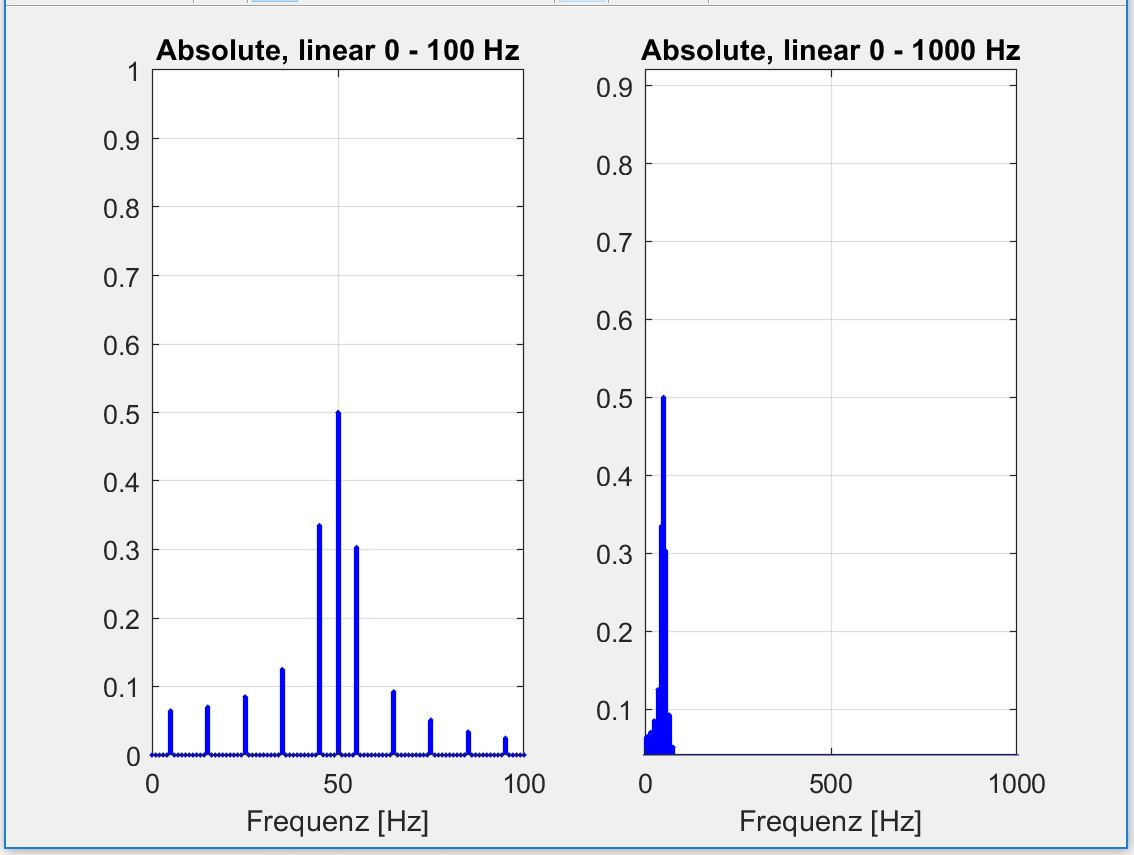
\includegraphics[width=0.45\linewidth]{Oberwellen_0_5.png}\label{fig:Schwingungspacketspektrum 0.5}}\qquad
	\subfloat[][]{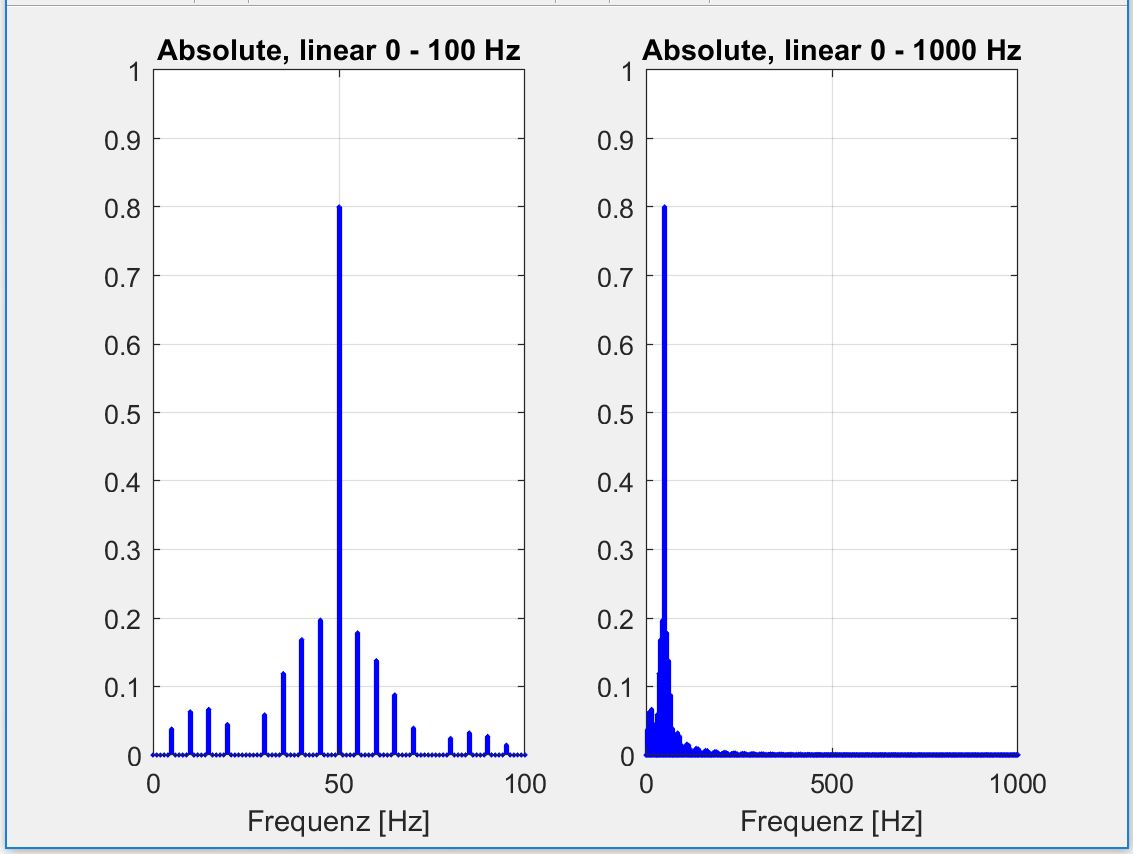
\includegraphics[width=0.45\linewidth]{Oberwellen_0_8.png}\label{fig:Schwingungspacketspektrum 0.8}}
	\caption{Lineares absolutes Spektrum mit einem duty cycle von (a) 0.5 (b) 0.8}
	\label{fig:Schwingungspaketspektrum Matlab}
\end{figure}

Schlussendlich untersuchte man noch den absoluten Logarithmus der beiden Funktionen. Die ist in der Abbildung \ref{fig:absolut_logaritmic_matlab} zu erkennen. Die y-Achse zeigt das Verhältnis der Spannungen an, dies wird immer in Dezibel angegeben. Bei der x-Achse handelt es sich um die Frequenz welche man untersucht hat. Auch hier wurde der absolute Logarithmus mit den zwei duty cycle 0.5 \ref{fig:absolut_logarithmic_0.5} und 0.8 \ref{fig:absolut_logarithmic_0.8} untersucht.


\begin{figure}[ht!]
	\centering
	\subfloat[][]{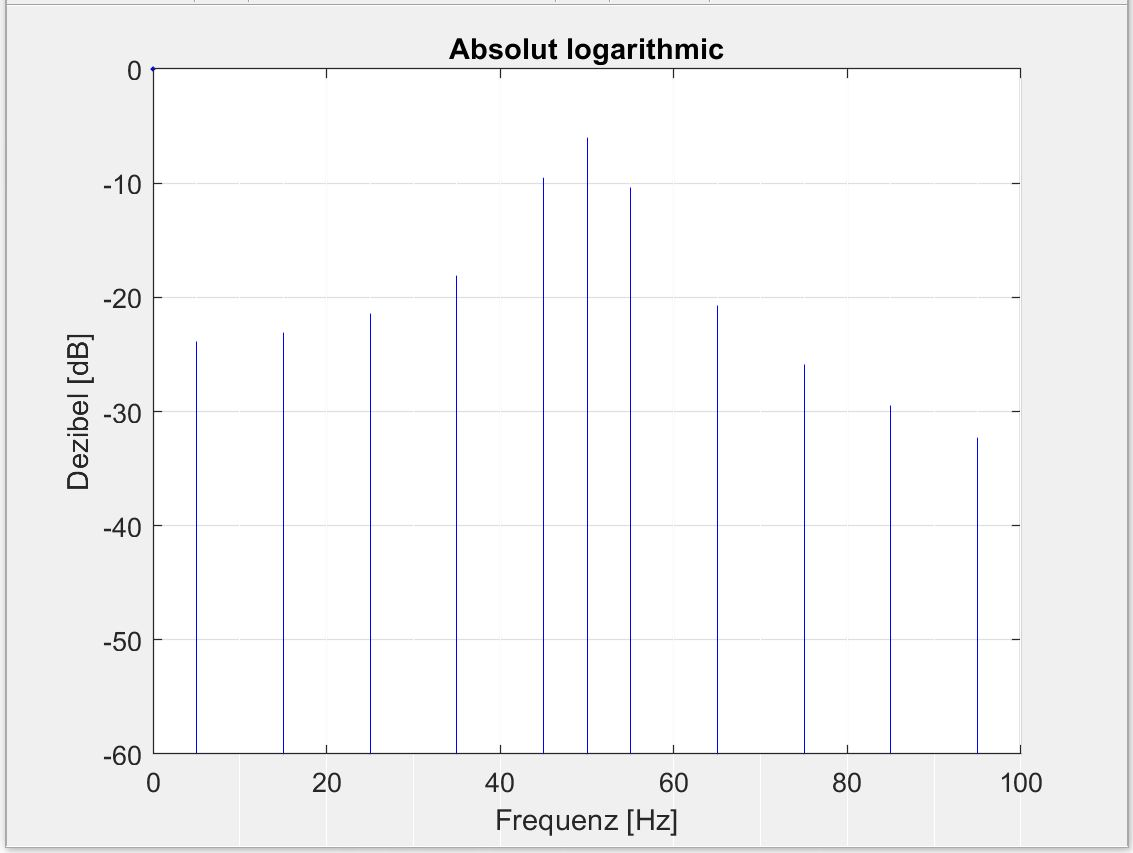
\includegraphics[width=0.45\linewidth]{absolut_logaritmic_0_5.png}\label{fig:absolut_logarithmic_0.5}}\qquad
	\subfloat[][]{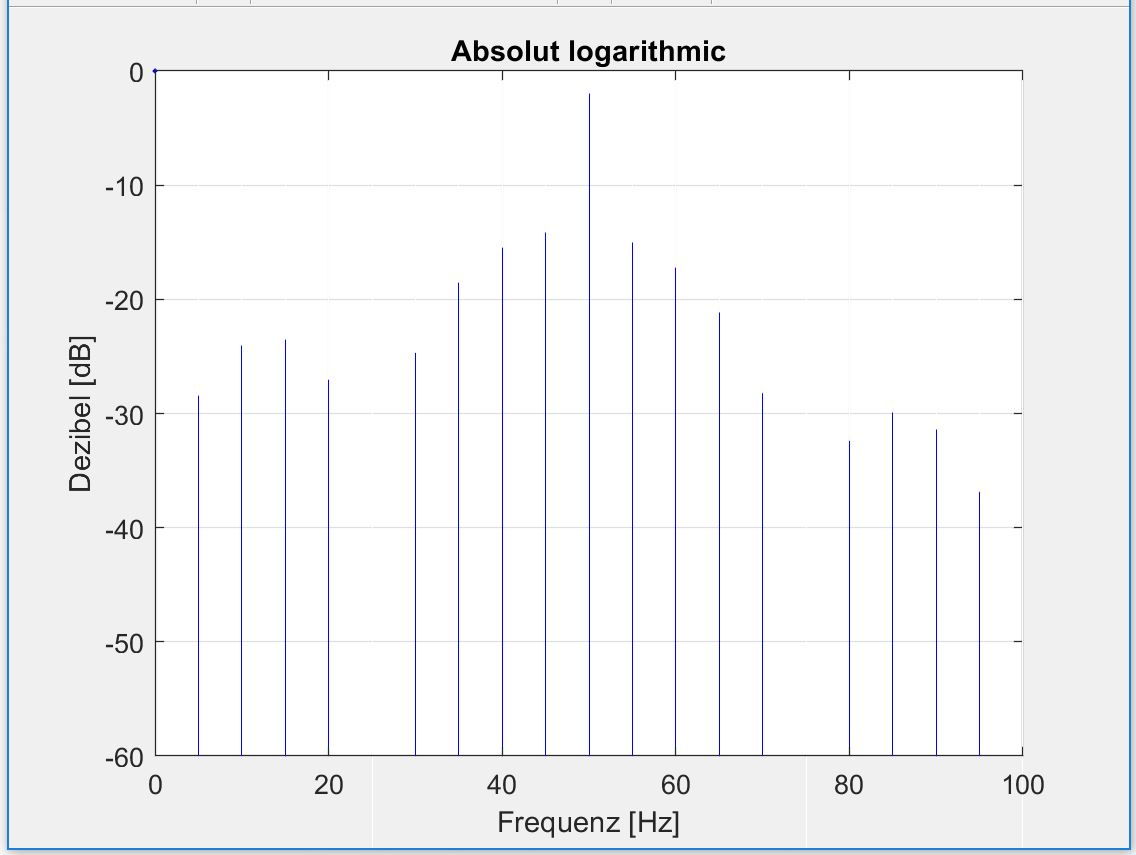
\includegraphics[width=0.45\linewidth]{absolut_logaritmic_0_8.png}\label{fig:absolut_logarithmic_0.8}}
	\caption{Lineares absolutes Spektrum mit einem duty cycle von (a) 0.5 (b) 0.8}
	\label{fig:absolut_logaritmic_matlab}
\end{figure}
\newpage
\subsection{Simulation mit Plecs}

Mit dem Simulationsprogramm Plecs konnte man alle gewünschten Ansteuerungen simulieren. Die einphasigen Simulationen der Phasenanschnitt- und der Schwingungspaketsteuerung wurden mit den Matlab-Funktionen verglichen und so auf ihre Richtigkeit überprüft. Nach dem man dies verifiziert hat, stellte man Verfahren für den dreiphasigen Phasenanschnitt- und Schwingungspaketsteuerung her. Ausserdem konstruierte man Kombinationen der beiden Verfahren im einphasigen und dreiphasigen System.\todo{alle Verfahren auflisten} Die Resultate sind auf den folgenden Seiten aufgezeigt.

\newpage

Auch bei der Plecs-Simulationen wurde als erstes die Phasenanschnittsteuerung untersucht. Gleich wie bei der Matlab-Simulation konnten die verschiedenen Winkeln des Anschnittes nach Belieben eingestellt werden. Um die Resultate verifizieren zu könne wählte man die selben Winkel wie in der Abbildung \ref{fig:eingangssignal_mit_Matlab}. In der unteren Grafik, erkennt man ein Sinussignal mit einem Phasenanschnitt von $60^\circ$ \ref{fig:plecs_eingangssignal_60} und einen mit $90^\circ$ \ref{fig:plecs_eingangssignal_90}. Um die Spektren mit den Matlab-Simulationen vergleichen zu können wurde die Amplitude des Sinussignales wieder auf ± 1 eingestellt. 

\begin{figure}[ht!]
	\centering
	\subfloat[][]{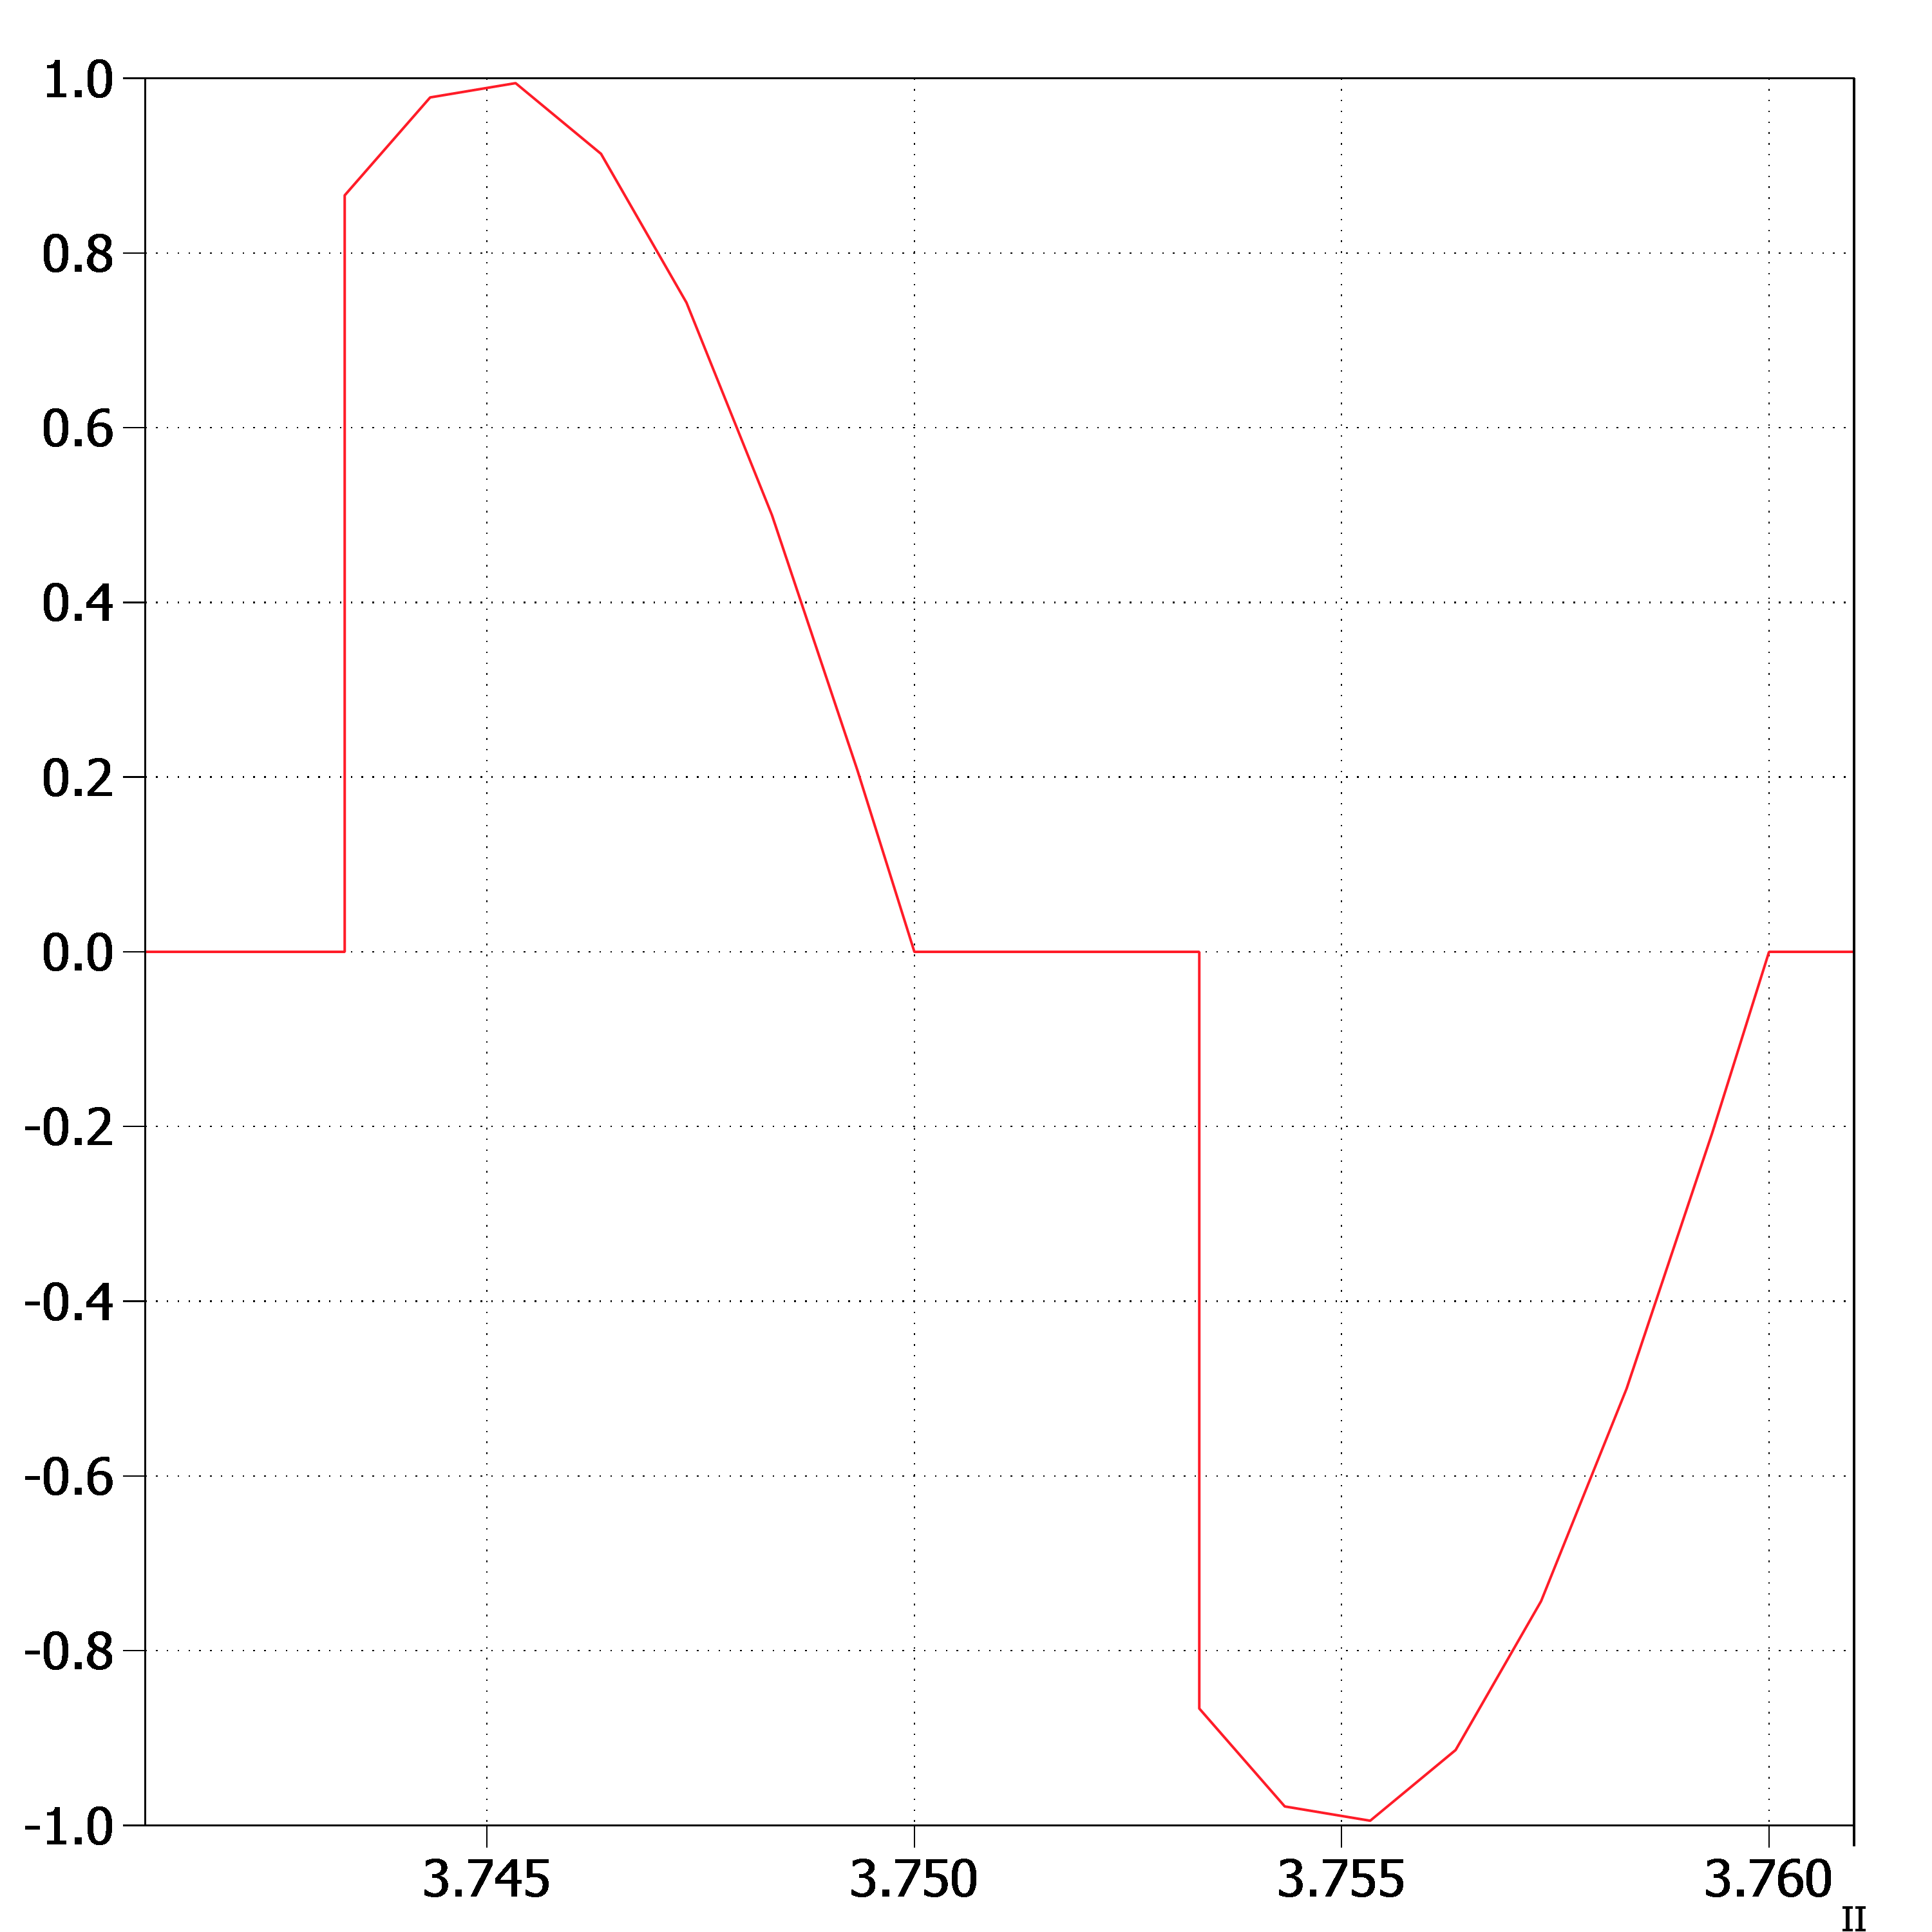
\includegraphics[width=0.43\linewidth]{plecs_phasenanschnitt_pi_3_funktion.png}\label{fig:plecs_eingangssignal_60}}\qquad
	\subfloat[][]{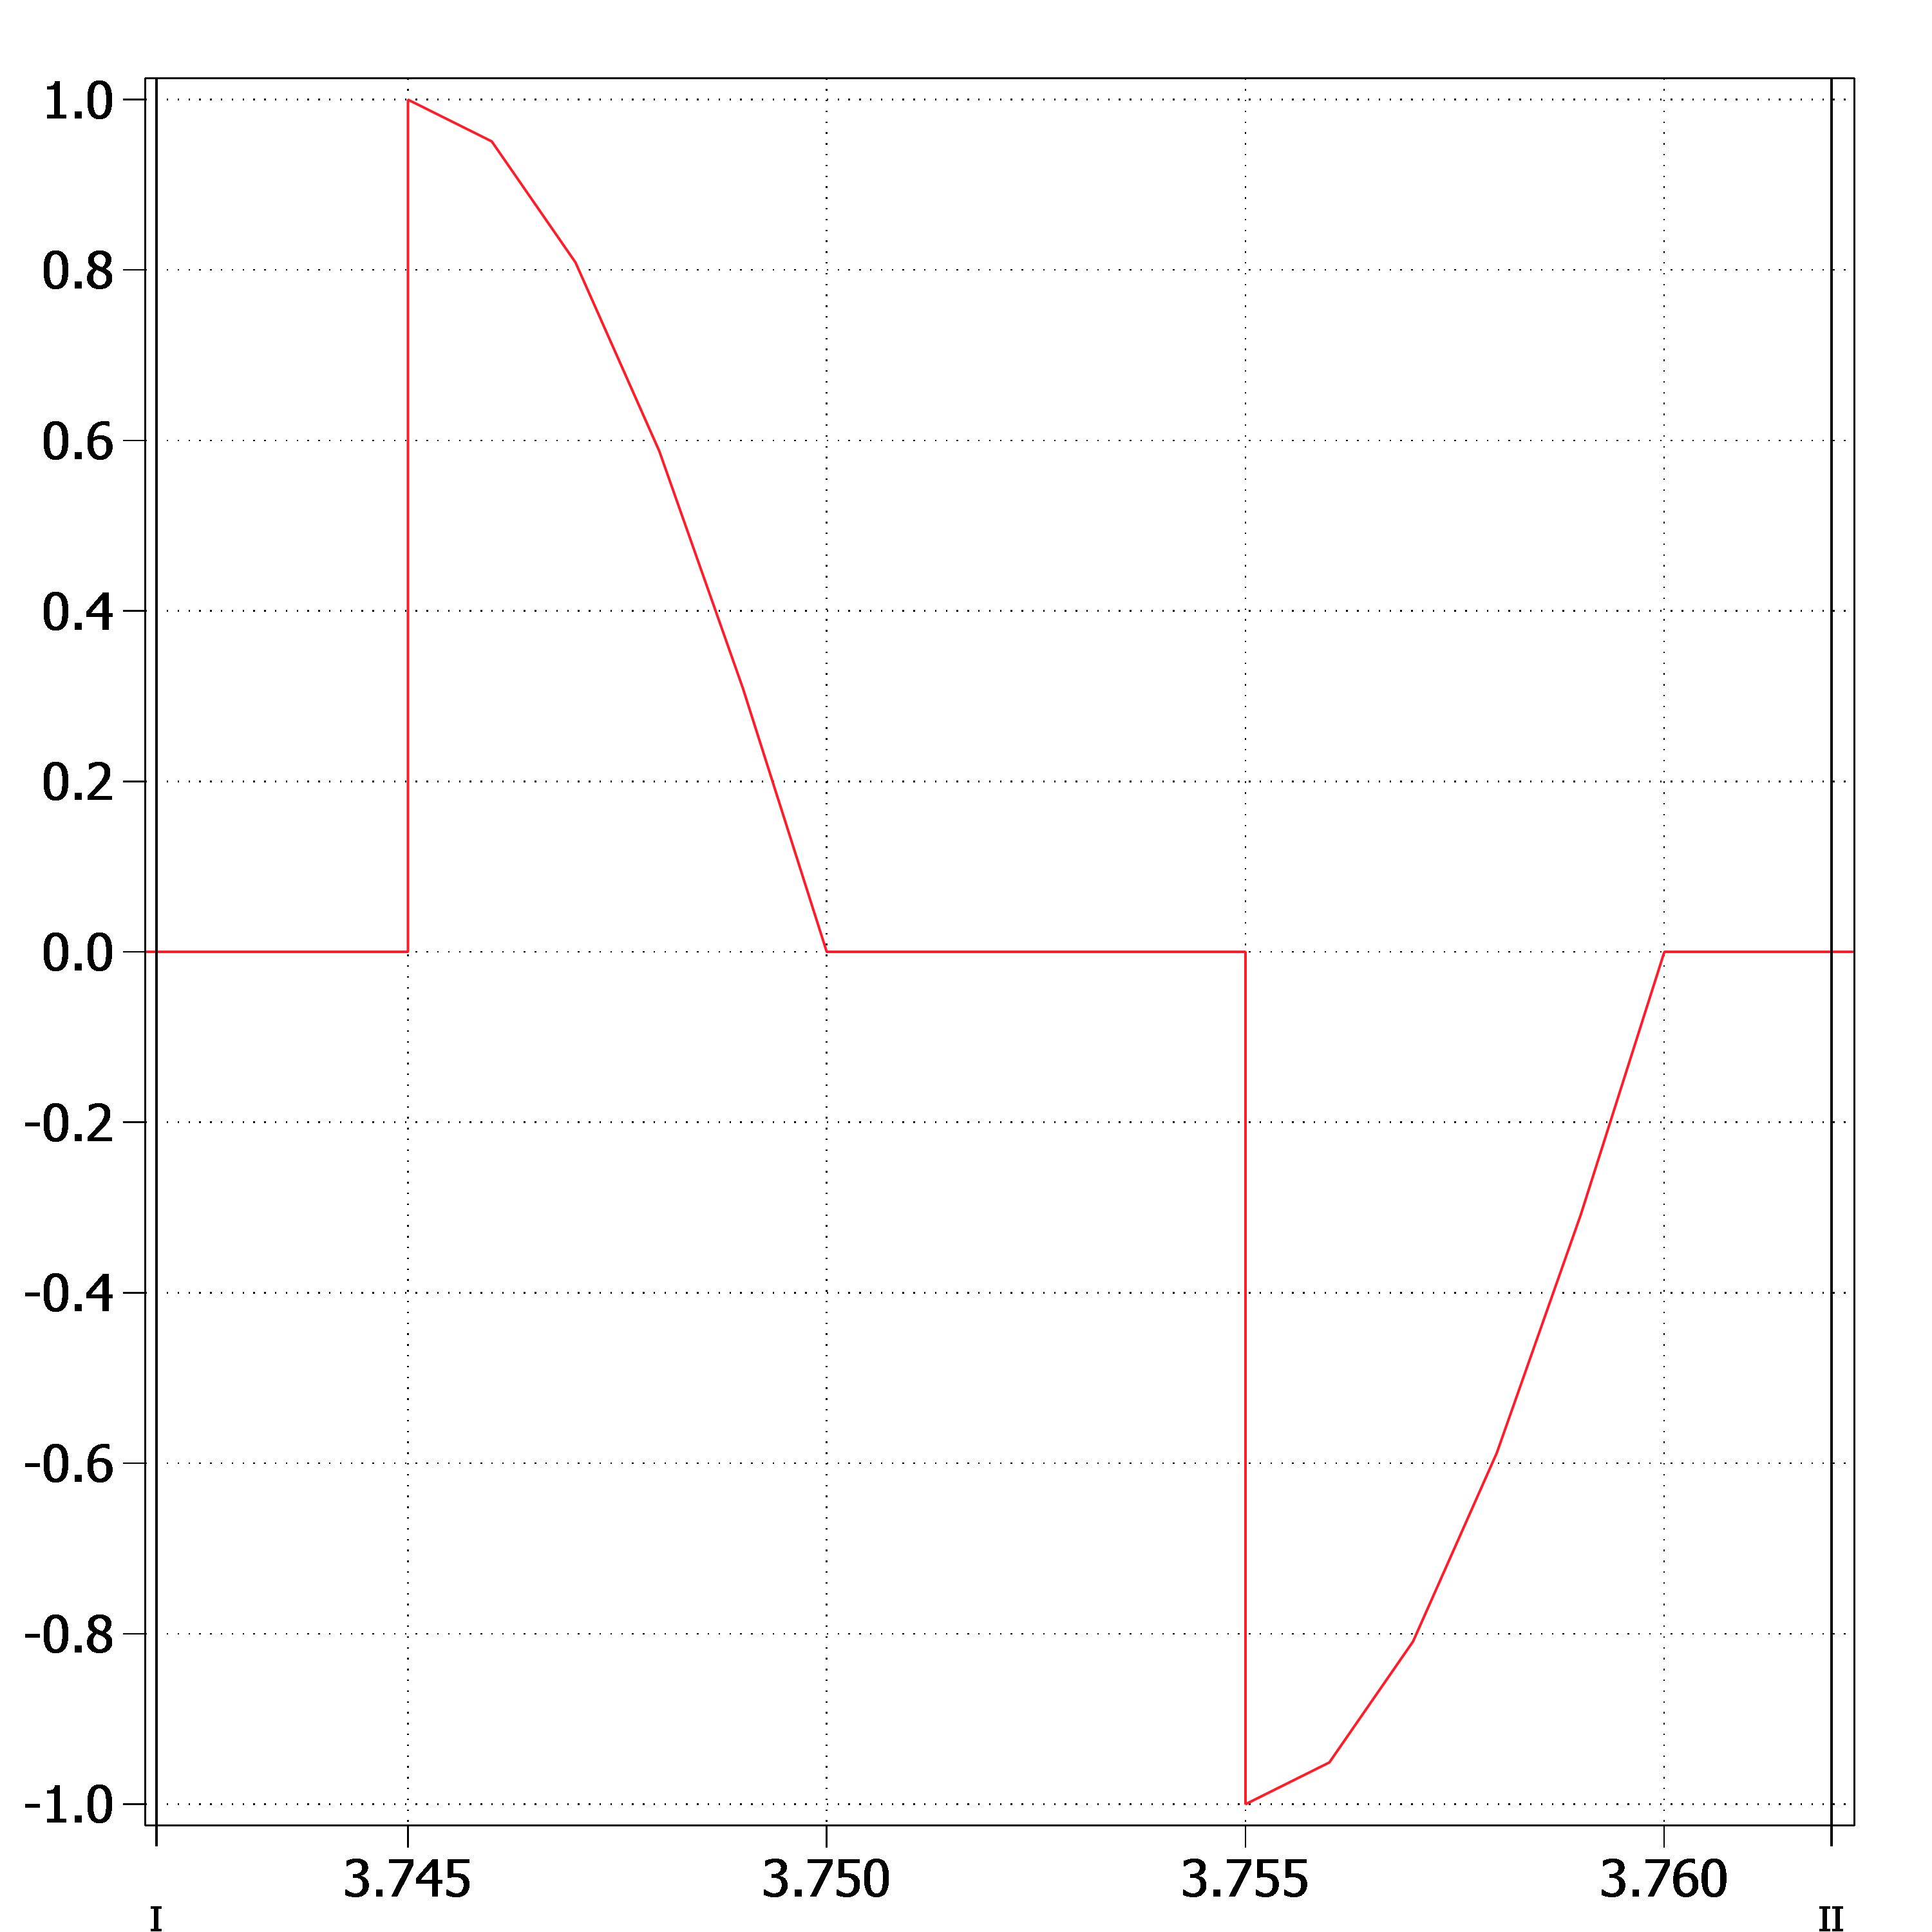
\includegraphics[width=0.43\linewidth]{plecs_phasenanschnitt_pi_2_funktion.png}\label{fig:plecs_eingangssignal_90}}
	\caption{Eingangssignal mit Phasenanschnitt (a) 60° (b) 90°}
	\label{fig:Eingangssignal simuliert mit Plecs}
\end{figure}

Die folgenden Bilder \ref{fig:plecs_Amplitudenspektrum} zeigen das Amplitudenspektrum der Phasenanschnittsteuerung mit den zwei bereits verwendeten Winkeln. Die Grafik musst nicht wie bei der Matlab-Funktion von Hand berechnet, sondern konnte mit Hilfe des Plecs Scope direkt analysiert werden. Plecs macht auch eine Fourier-Analyse um das Spektrum anzuzeigen. Vergleicht man die Amplitudenspektren der beiden Simulationen miteinander sehen die Grafiken, nach erster Einschätzung von Auge, sehr ähnlich aus. Der genau Vergleich der Werte wird weiter unten im Kapitel XX beschrieben.   
     
\begin{figure}[ht!]
	\centering
	\subfloat[][]{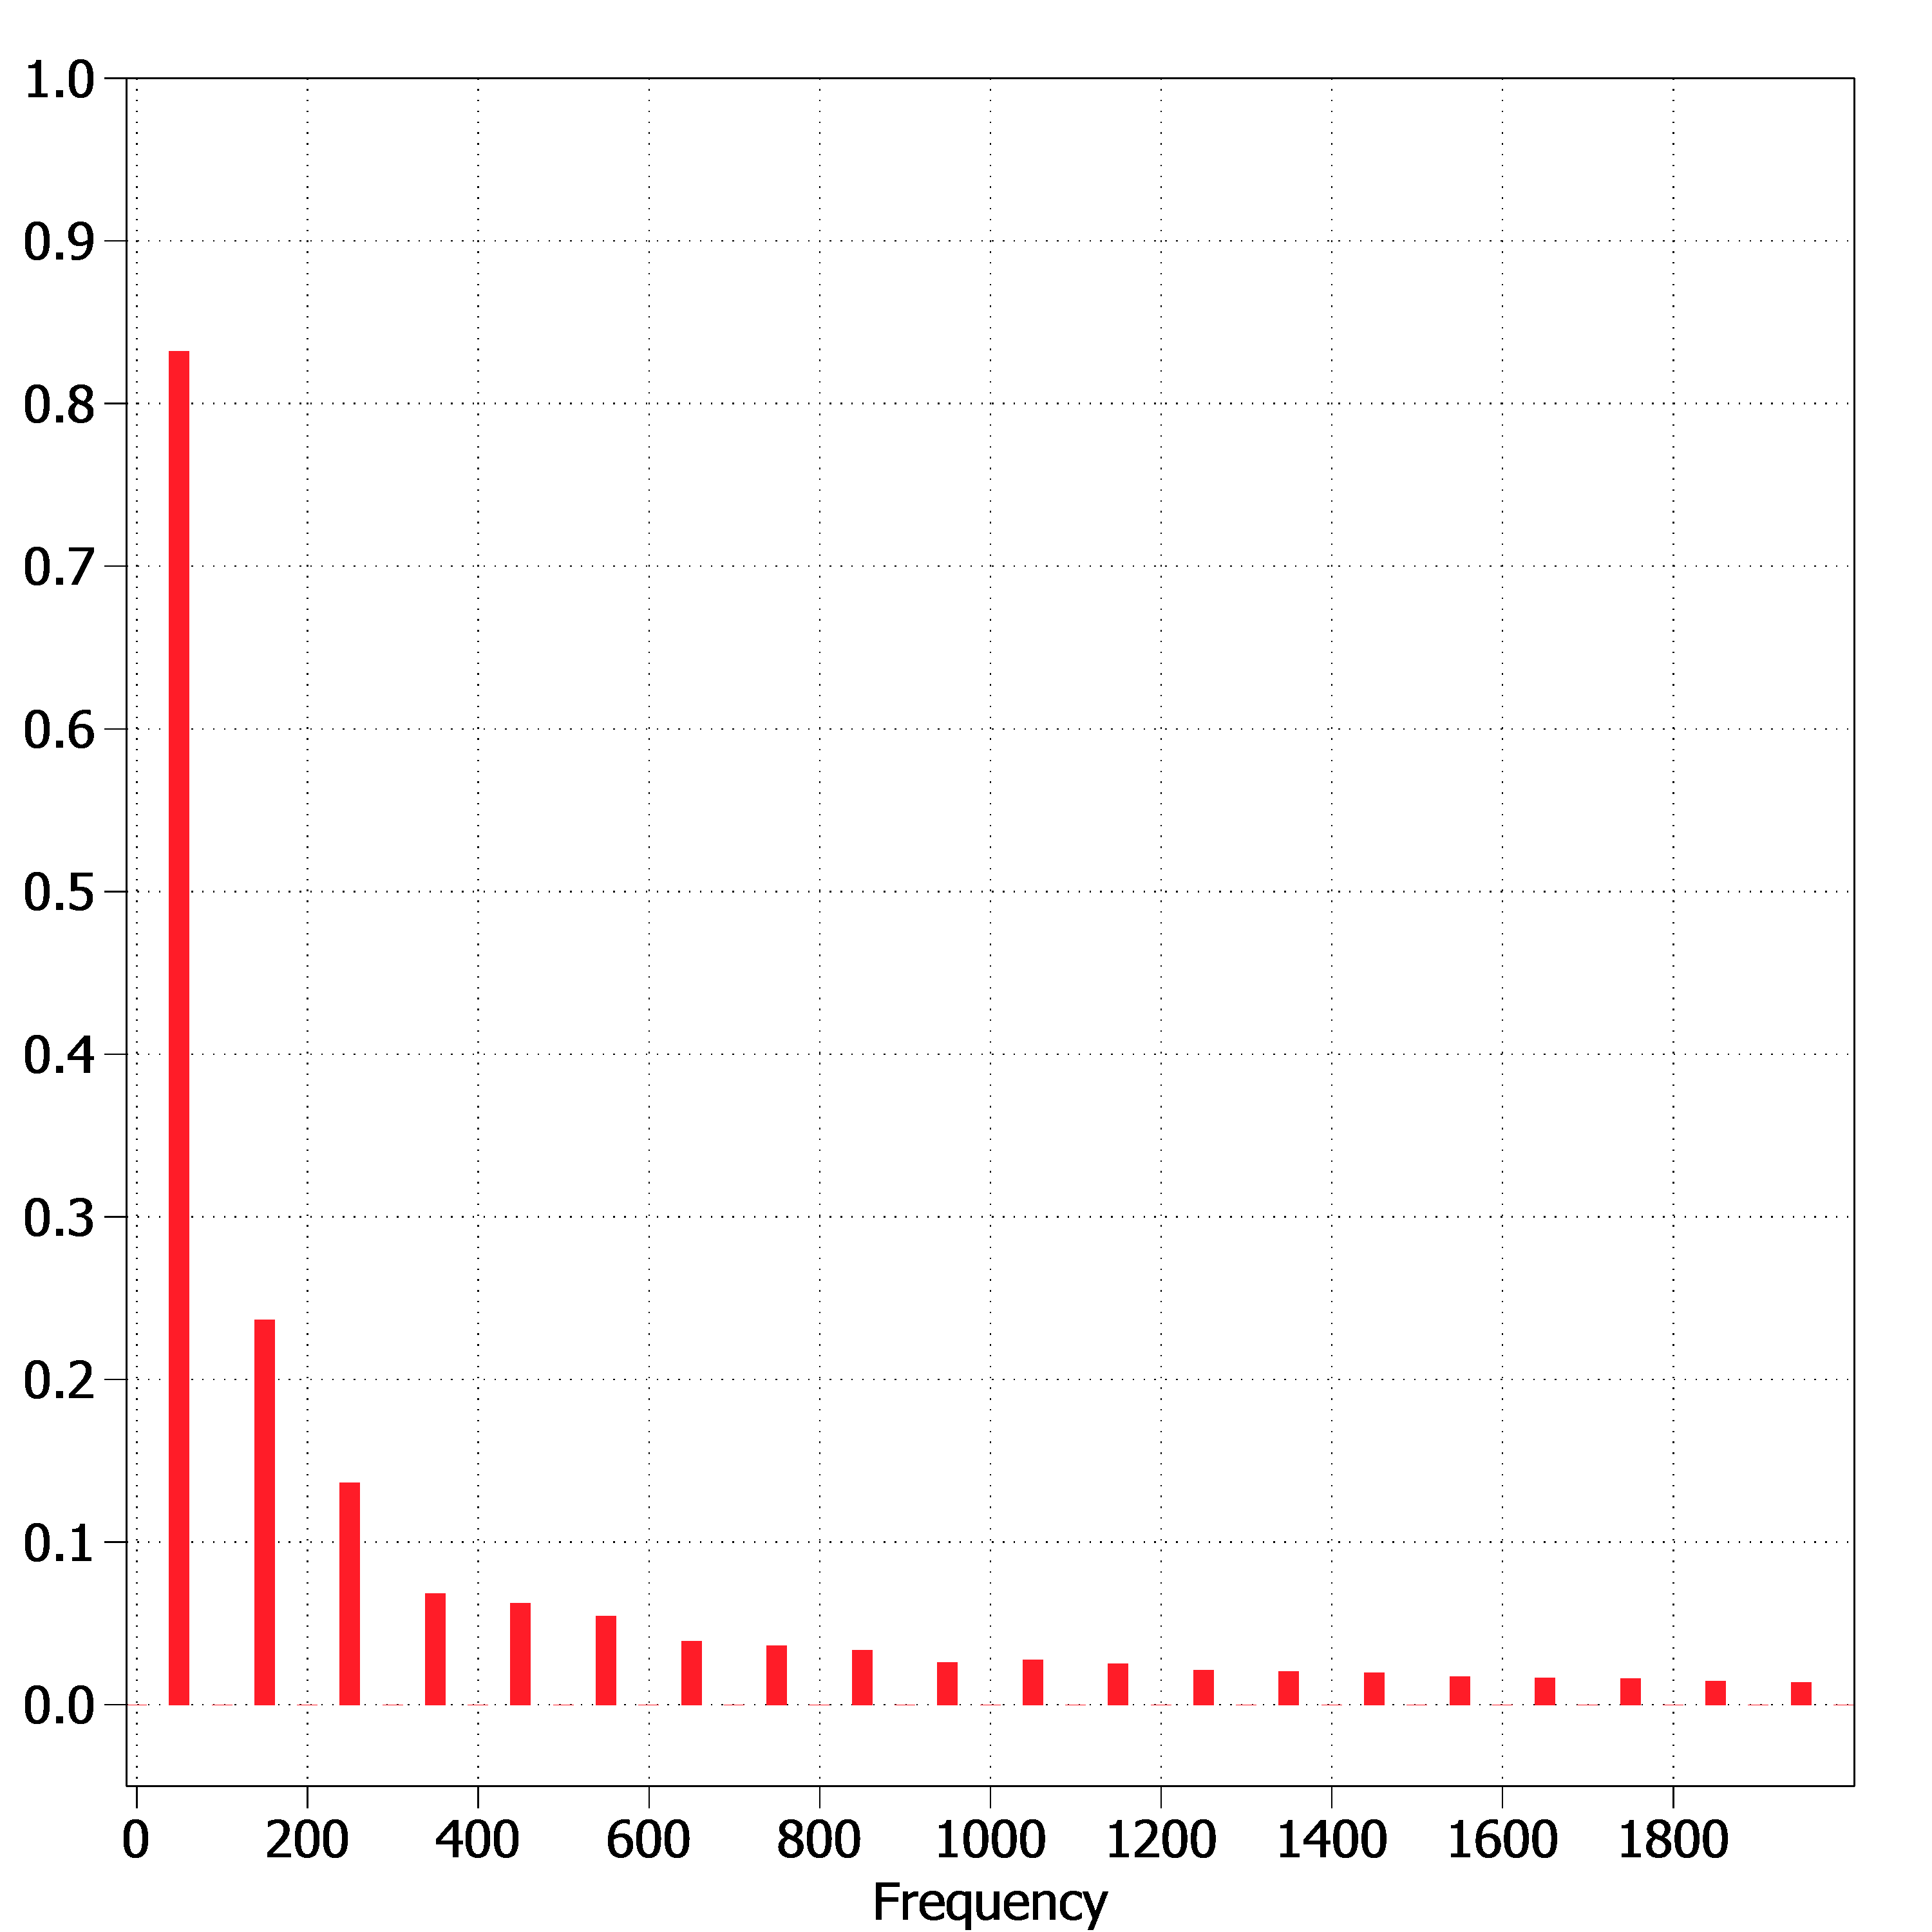
\includegraphics[width=0.43\linewidth]{plecs_phasenanschnitt_pi_3.png}\label{fig:plecs_Amplitudenspektrum_60}}\qquad
	\subfloat[][]{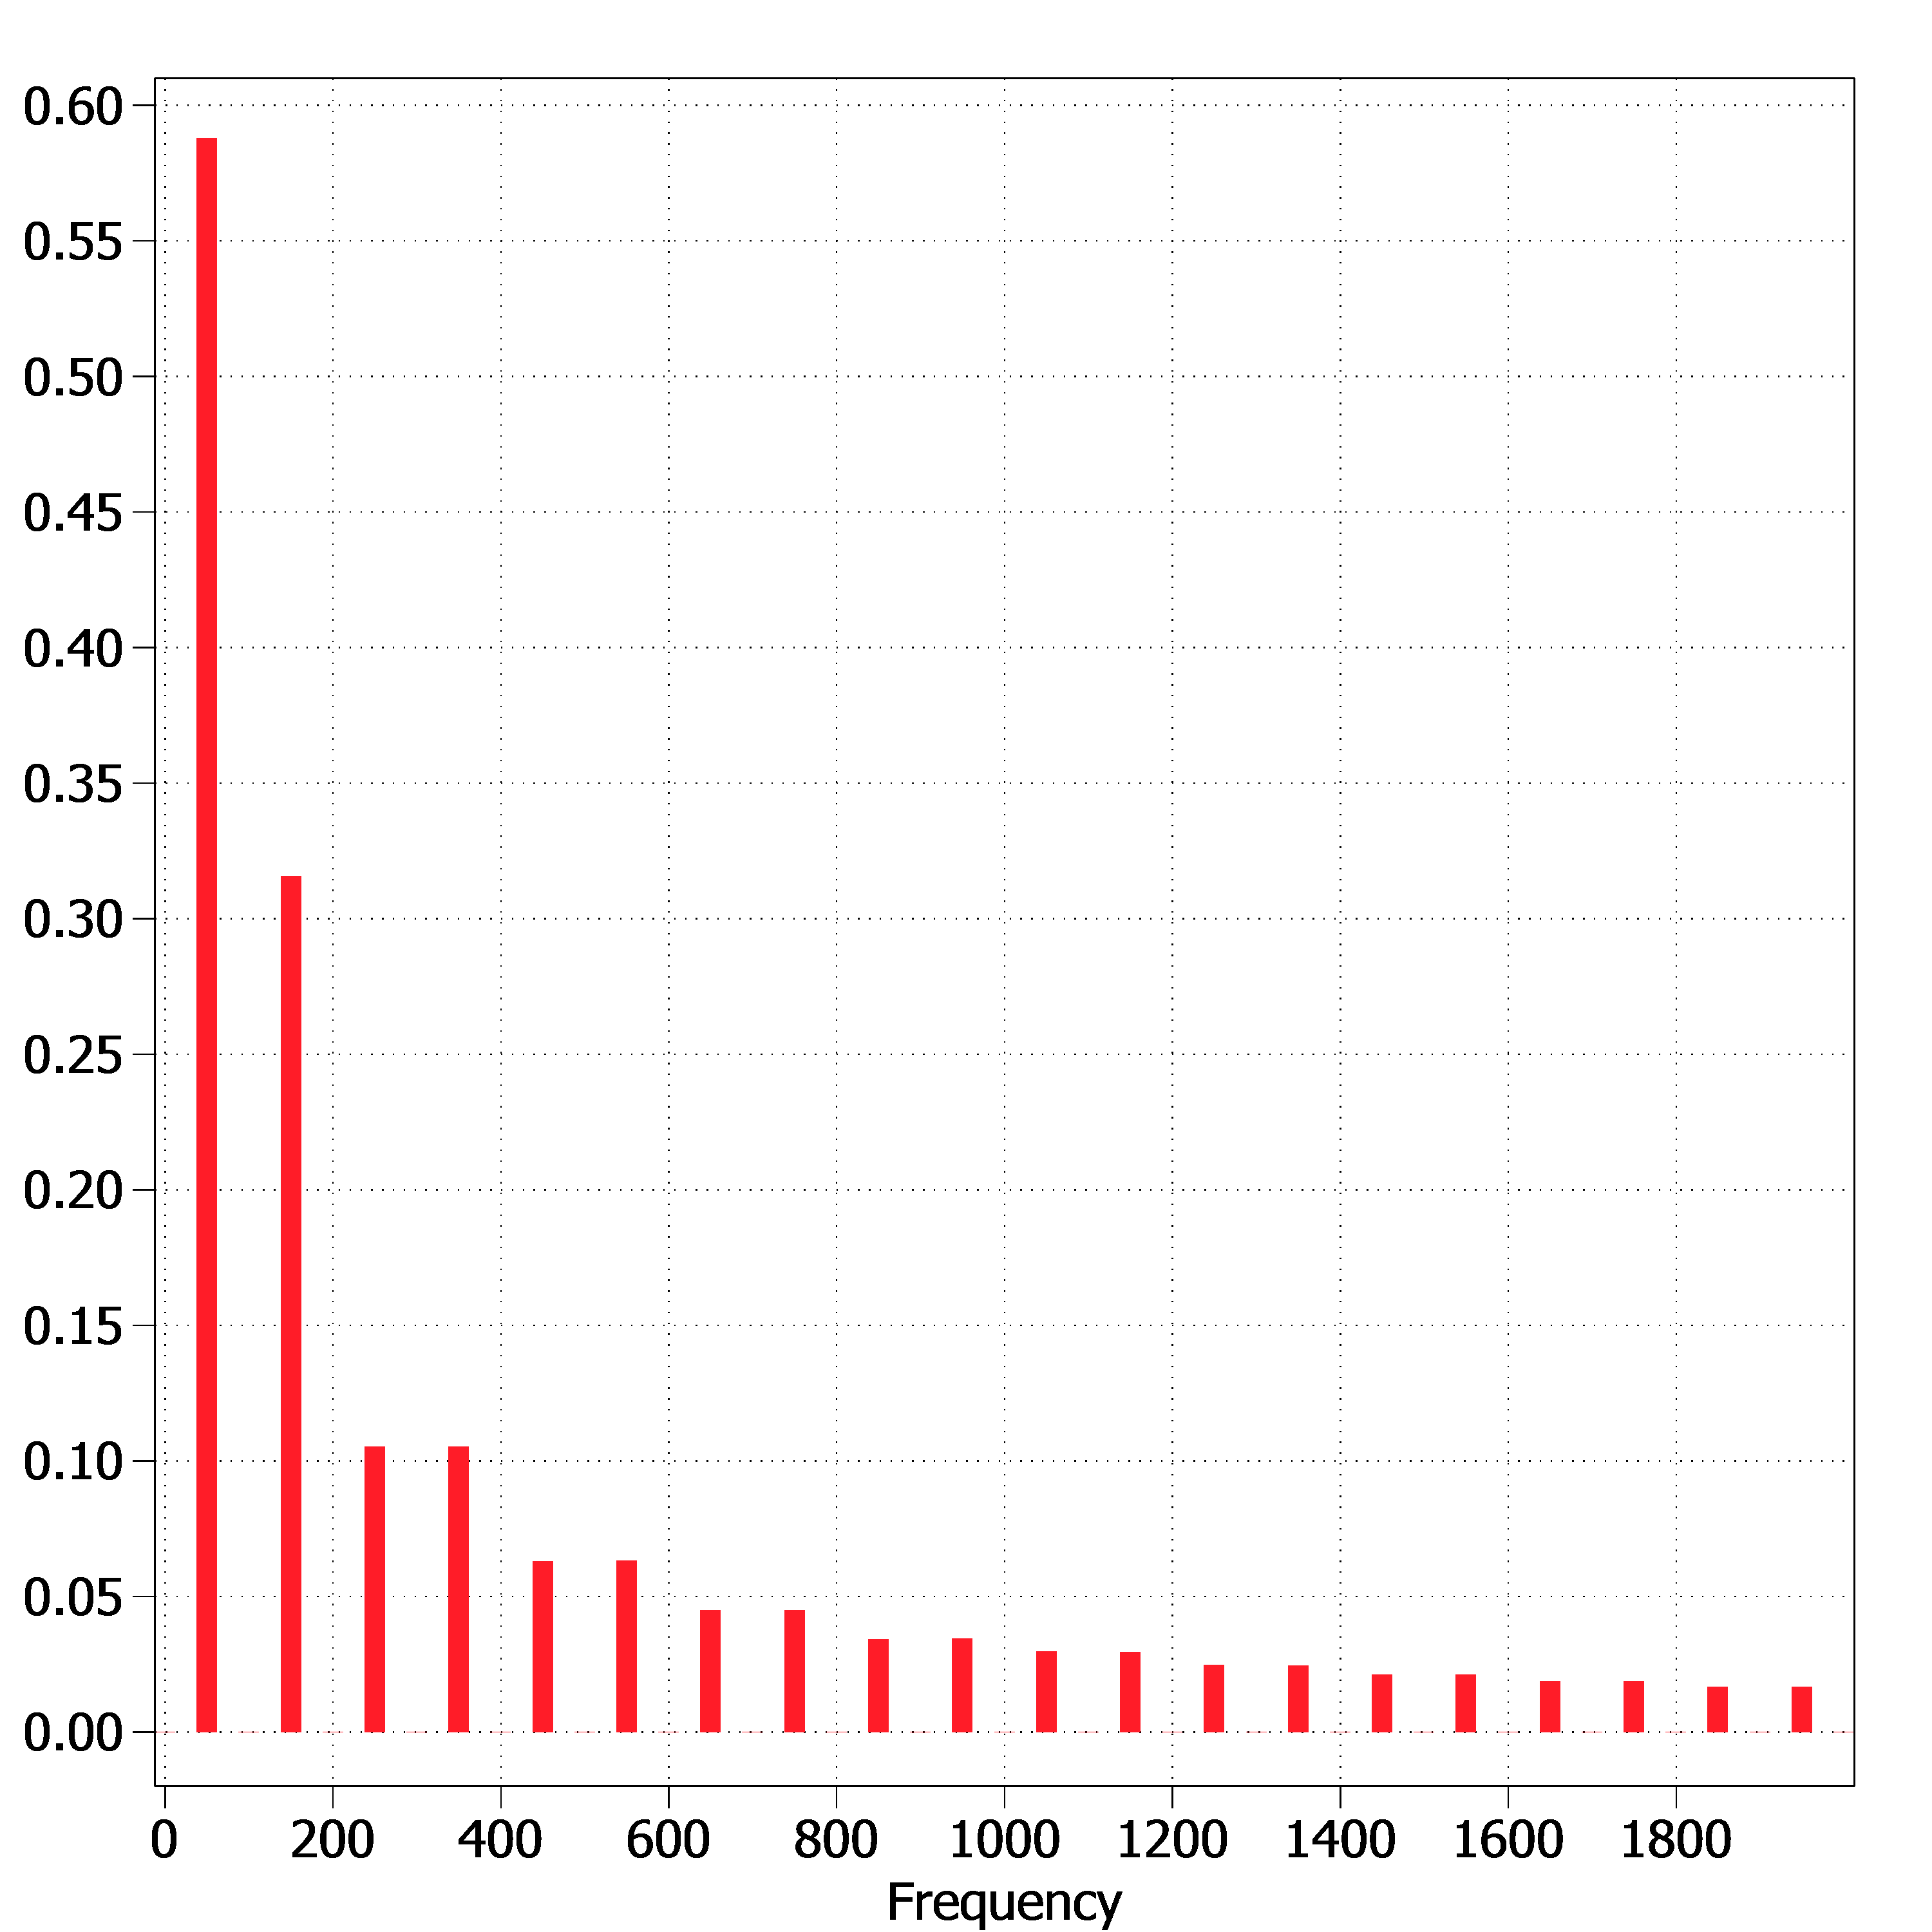
\includegraphics[width=0.43\linewidth]{plecs_phasenanschnitt_pi_2.png}\label{fig:plecs_Amplitudenspektrum_90}}
	\caption{Amplitudenspektrum (a) 60° (b) 90°}
	\label{fig:plecs_Amplitudenspektrum}
\end{figure}

Als nächstes wurde eine Simulation für die Schwingungspaketsteuerung aufgebaut. Auch hier verwendete man einen duty cycle von 0.5 \ref{fig:plecs_Schwingungspaket_0_5} beziehungsweise 0.8 \ref{fig:plecs_Schwingungspaket_0_8}. Die untere Abbildung \ref{fig:plecs_Schwingungspakete} zeigt beiden Signale.  
\begin{figure}[ht!]
	\centering
	\subfloat[][]{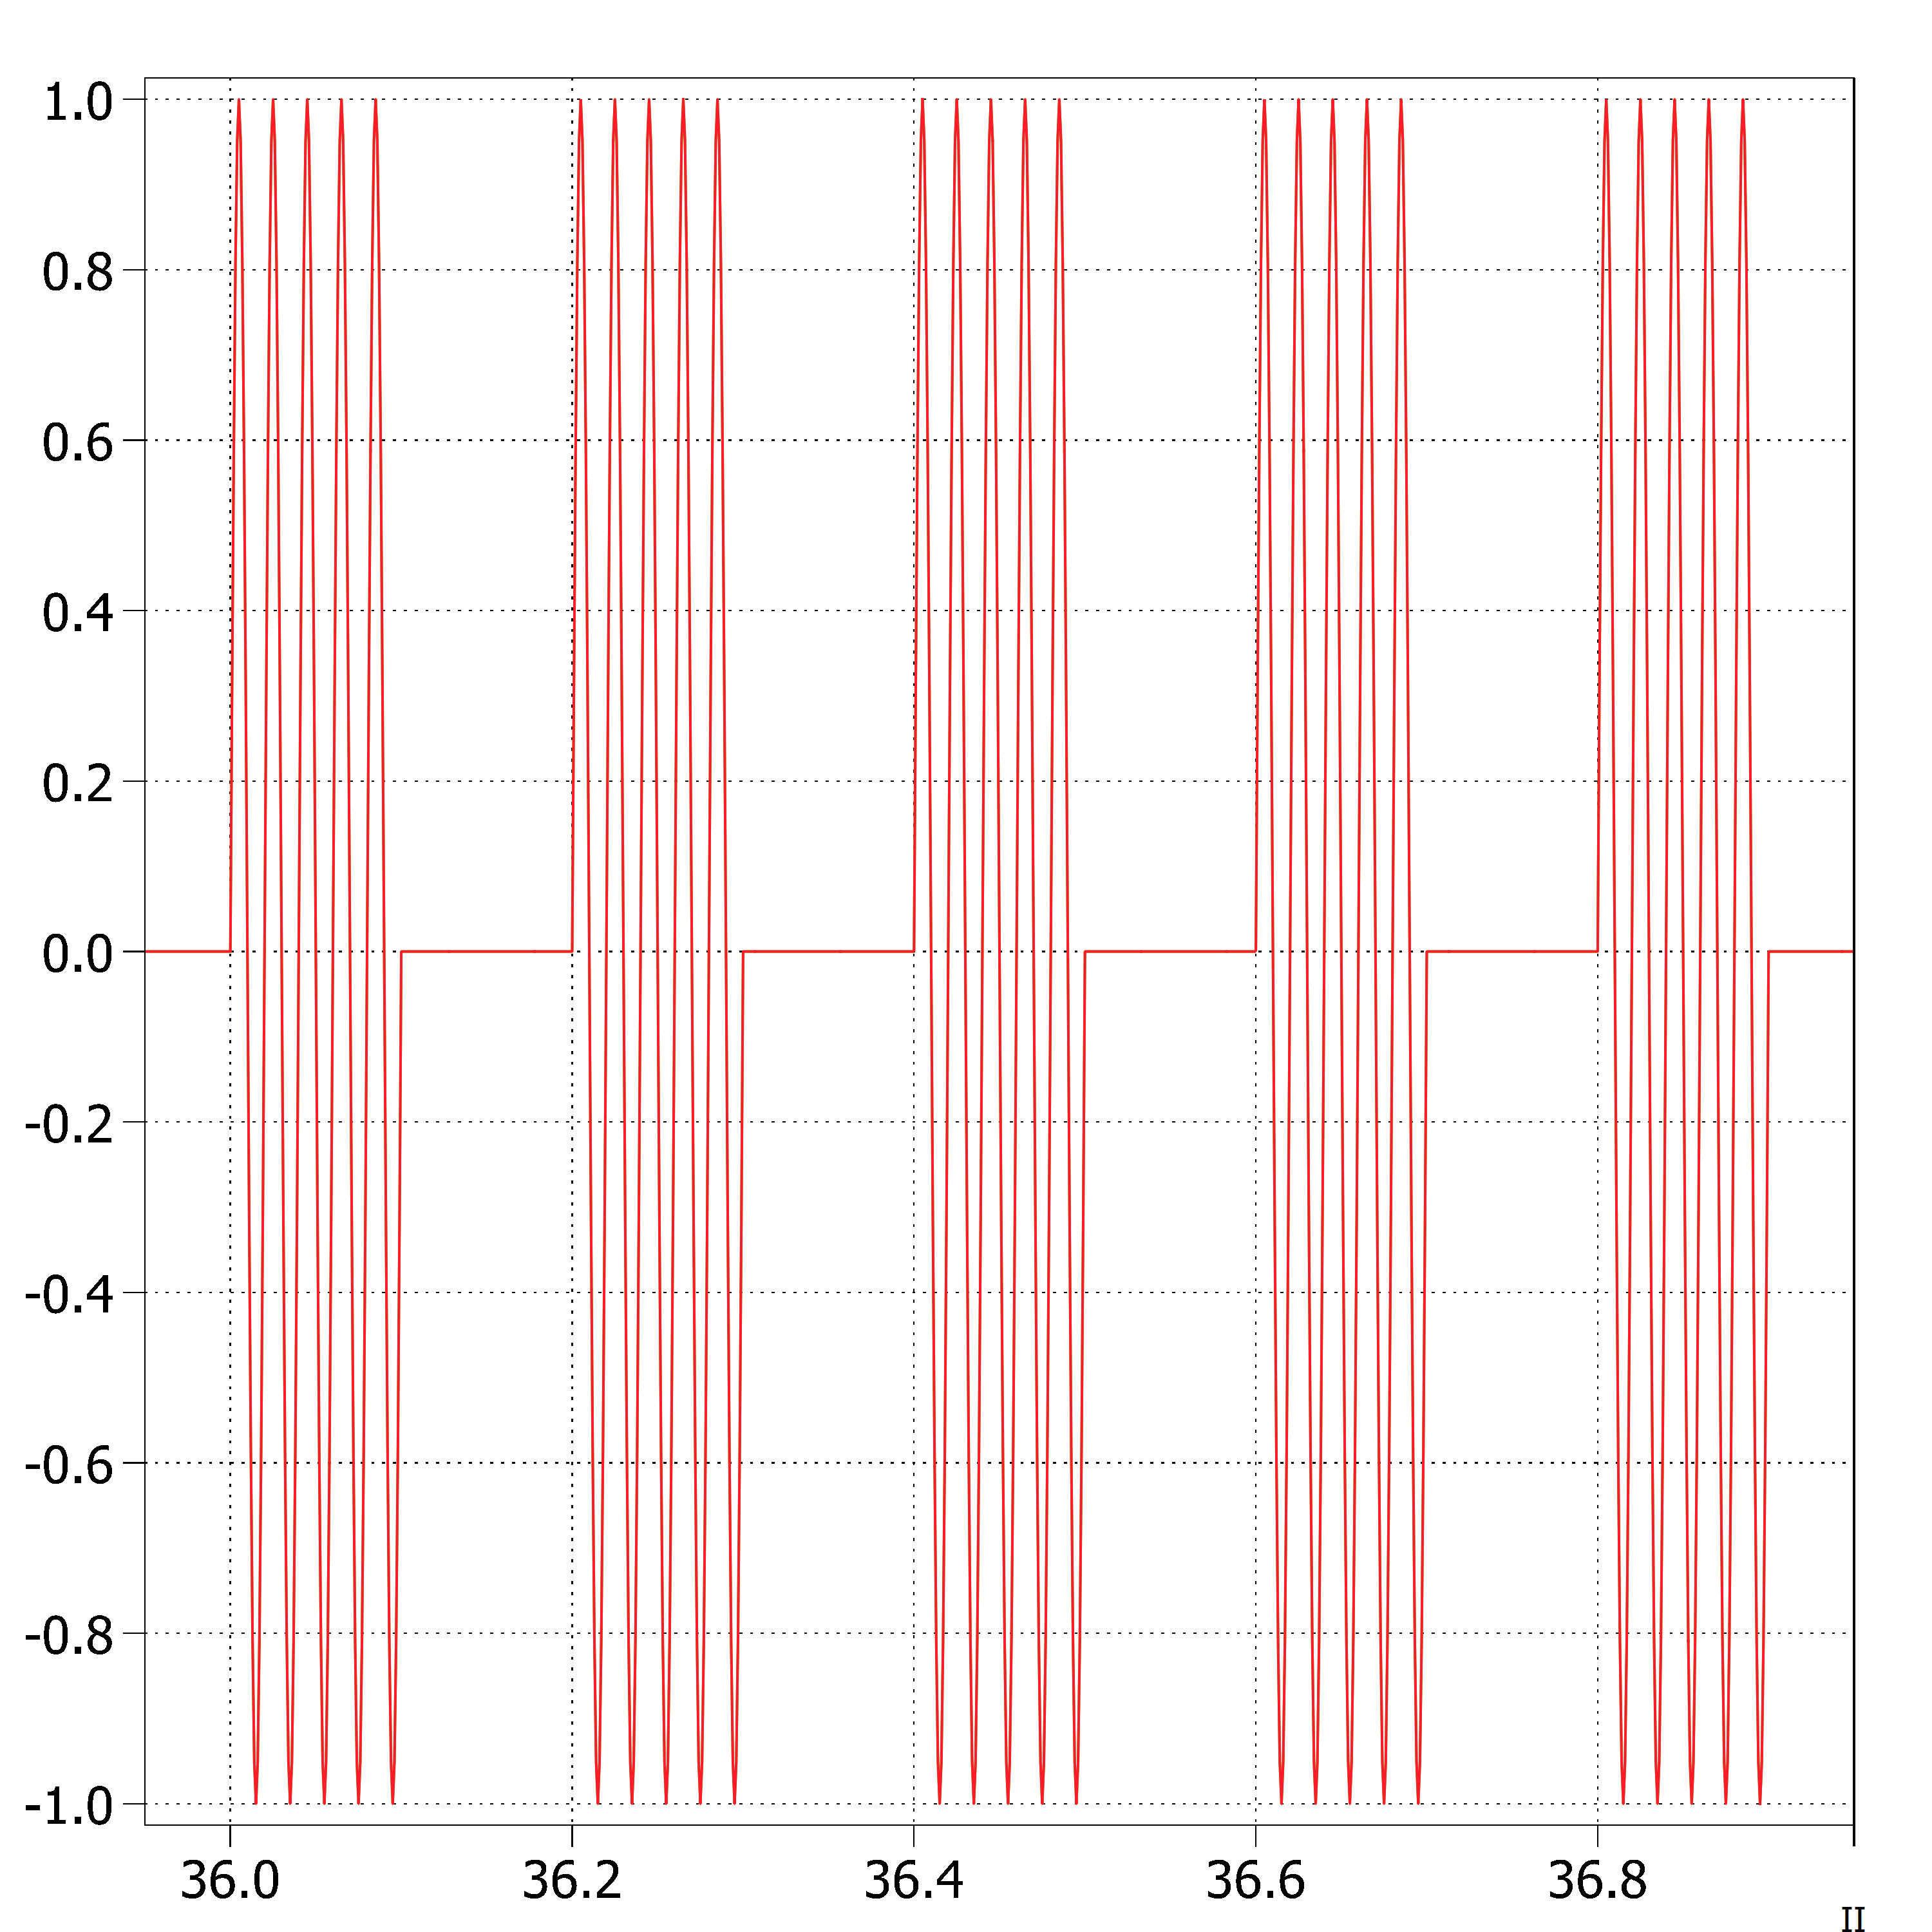
\includegraphics[width=0.45\linewidth]{plecs_schwingungspacket_0_5_schwingungen.PNG}\label{fig:plecs_Schwingungspaket_0_5}}\qquad
	\subfloat[][]{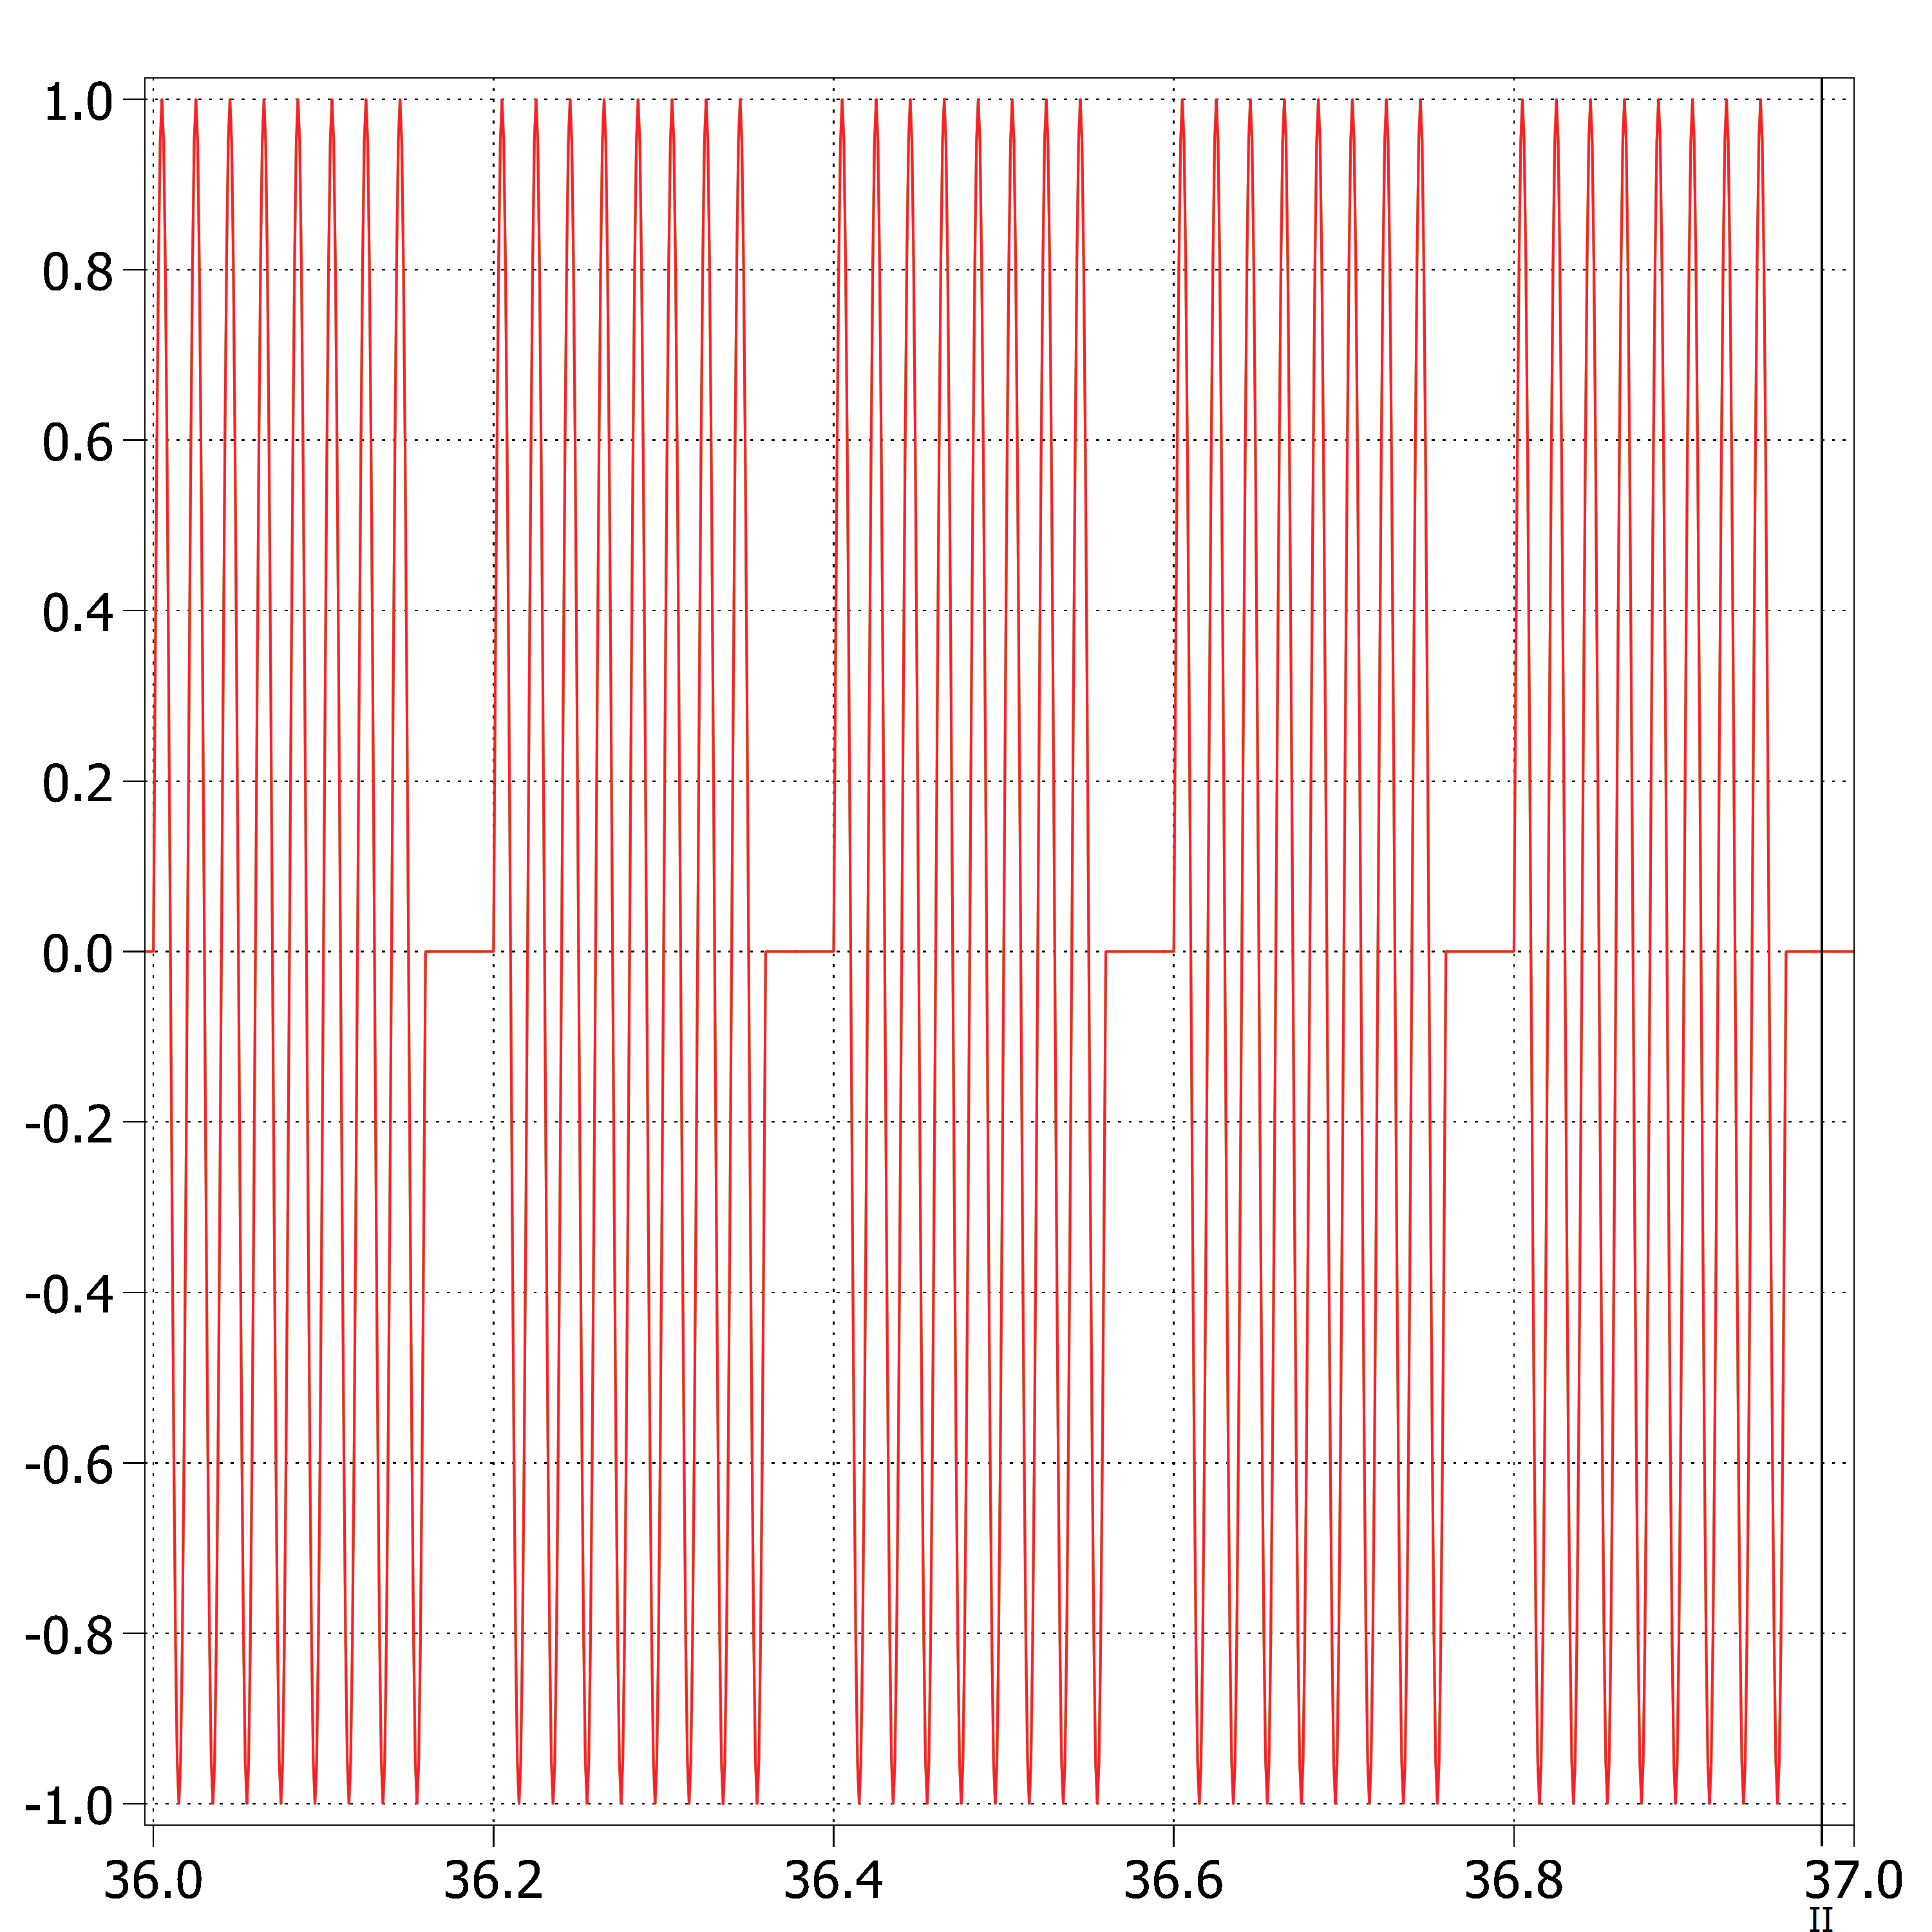
\includegraphics[width=0.45\linewidth]{plecs_schwingungspacket_0_8_schwingungen.PNG}\label{fig:plecs_Schwingungspaket_0_8}}
	\caption{Schwingungspaket mit einem duty cycle (a) 0.5 (b) 0.8}
	\label{fig:plecs_Schwingungspakete}
\end{figure}

In der folgende Abbildung \ref{fig:plecs_Schwingungspakete_Amplitudenspektrum_ 0_5_100_1000} wurde das Amplitudenspektrum des Schwingungspaketes mit einem duty cycle von 0.5 dargestellt. Auf der linken Seite \ref{fig:plecs_Schwingungspaket_0_5_100} der Abbildung erkennt man das bekannte Spektrum von 0- 100 Hz mit den Subharmonischen Werten unterhalb von 50 Hz. Rechts \ref{fig:plecs_Schwingungspaket_0_5_1000} davon ist das Spektrum bis zu 1000 Hz erweitert worden. Auch hier ist eine optische Ähnlichkeit zur  Matlab-Funktion ersichtlich.     
\begin{figure}[ht!]
	\centering
	\subfloat[][]{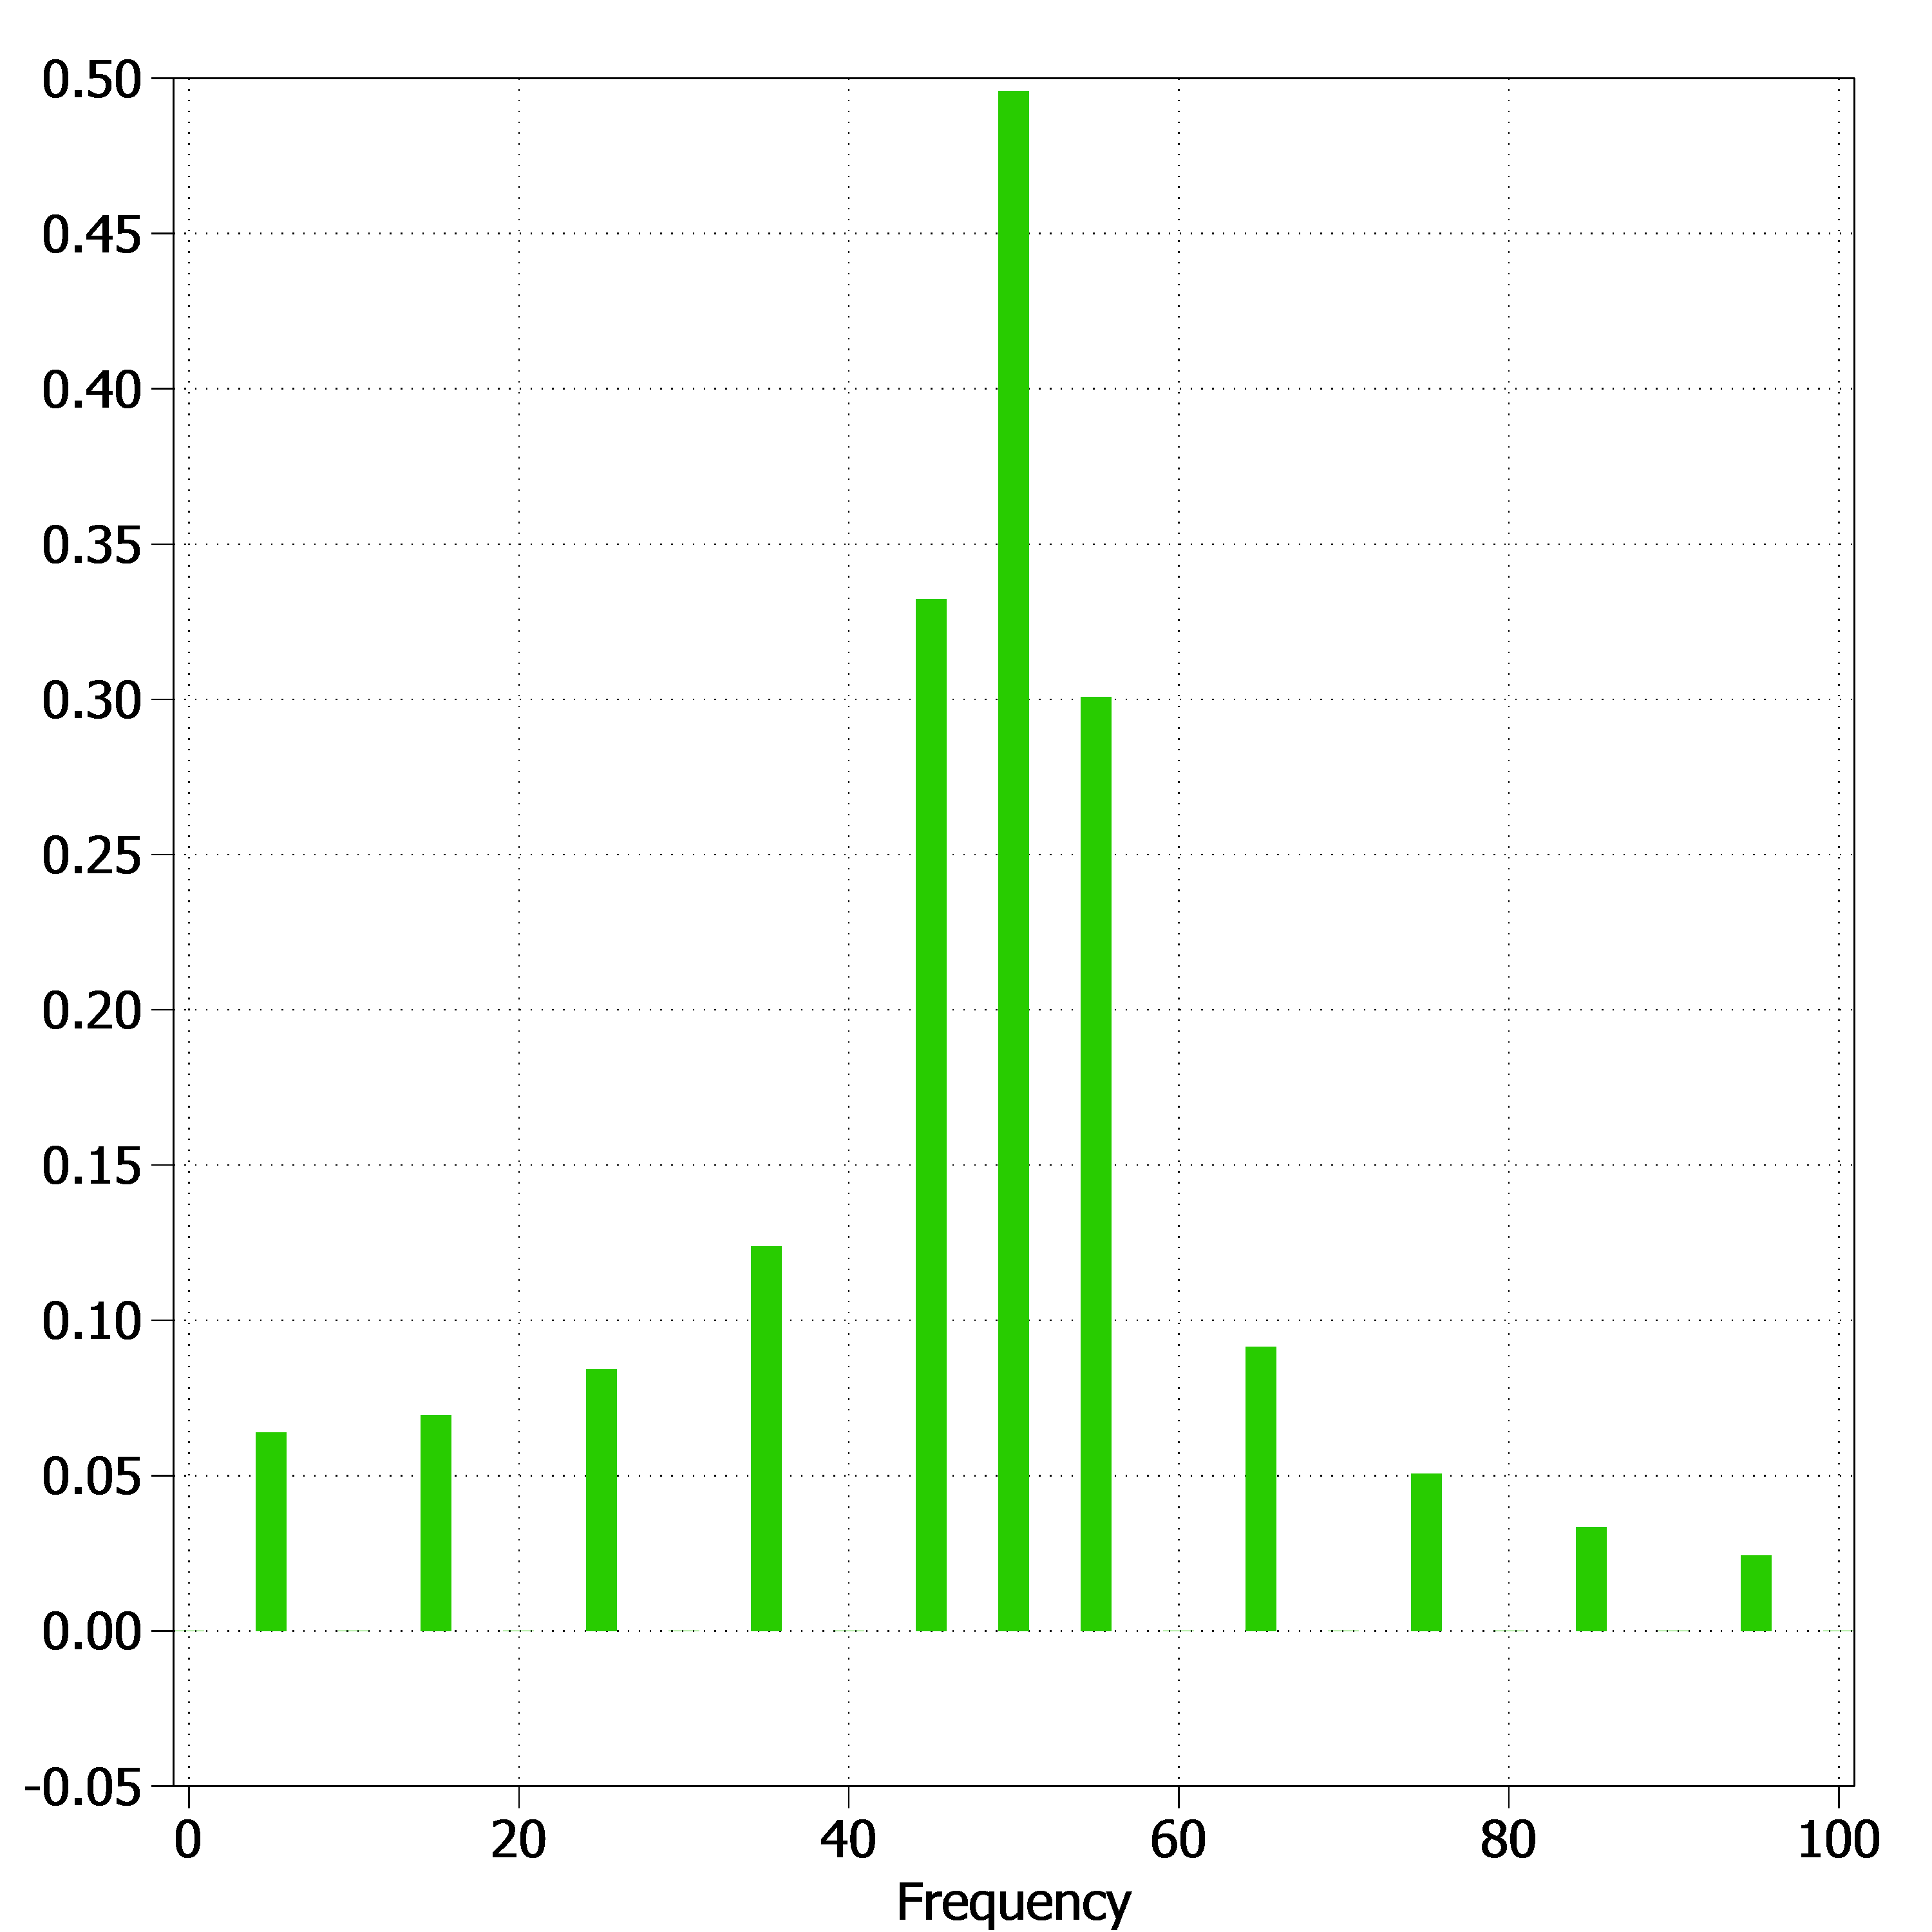
\includegraphics[width=0.45\linewidth]{plecs_schwingungspacket_0_5_100.PNG}\label{fig:plecs_Schwingungspaket_0_5_100}}\qquad
	\subfloat[][]{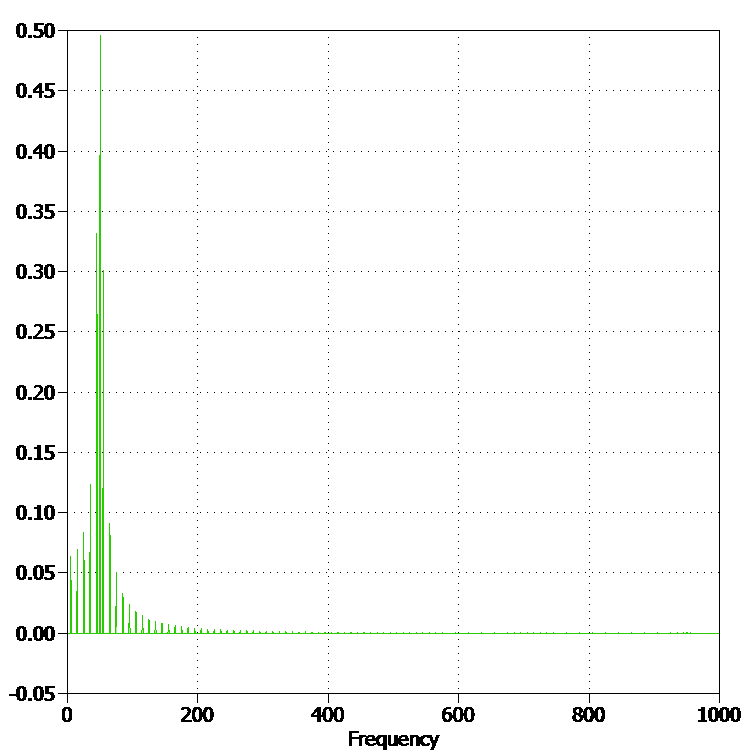
\includegraphics[width=0.45\linewidth]{plecs_schwingungspacket_0_5_1000.PNG}\label{fig:plecs_Schwingungspaket_0_5_1000}}
	\caption{Amplitudenspektrum mit einem duty cycle 0.5 von (a) 0 - 100 Hz (b) 0 - 1000 Hz}
	\label{fig:plecs_Schwingungspakete_Amplitudenspektrum_ 0_5_100_1000}
\end{figure}

Anschliessend wurde das gleiche noch mit dem duty cycle von 0.8 \ref{fig:plecs_Schwingungspakete_Amplitudenspektrum_ 0_8_100_1000} realisiert. Links \ref{fig:plecs_Schwingungspaket_0_8_100} wieder mit einer Frequenz von 0 - 100 Hz und rechts \ref{fig:plecs_Schwingungspaket_0_8_1000} das Spektrum bis 1000 Hz.
\begin{figure}[ht!]
	\centering
	\subfloat[][]{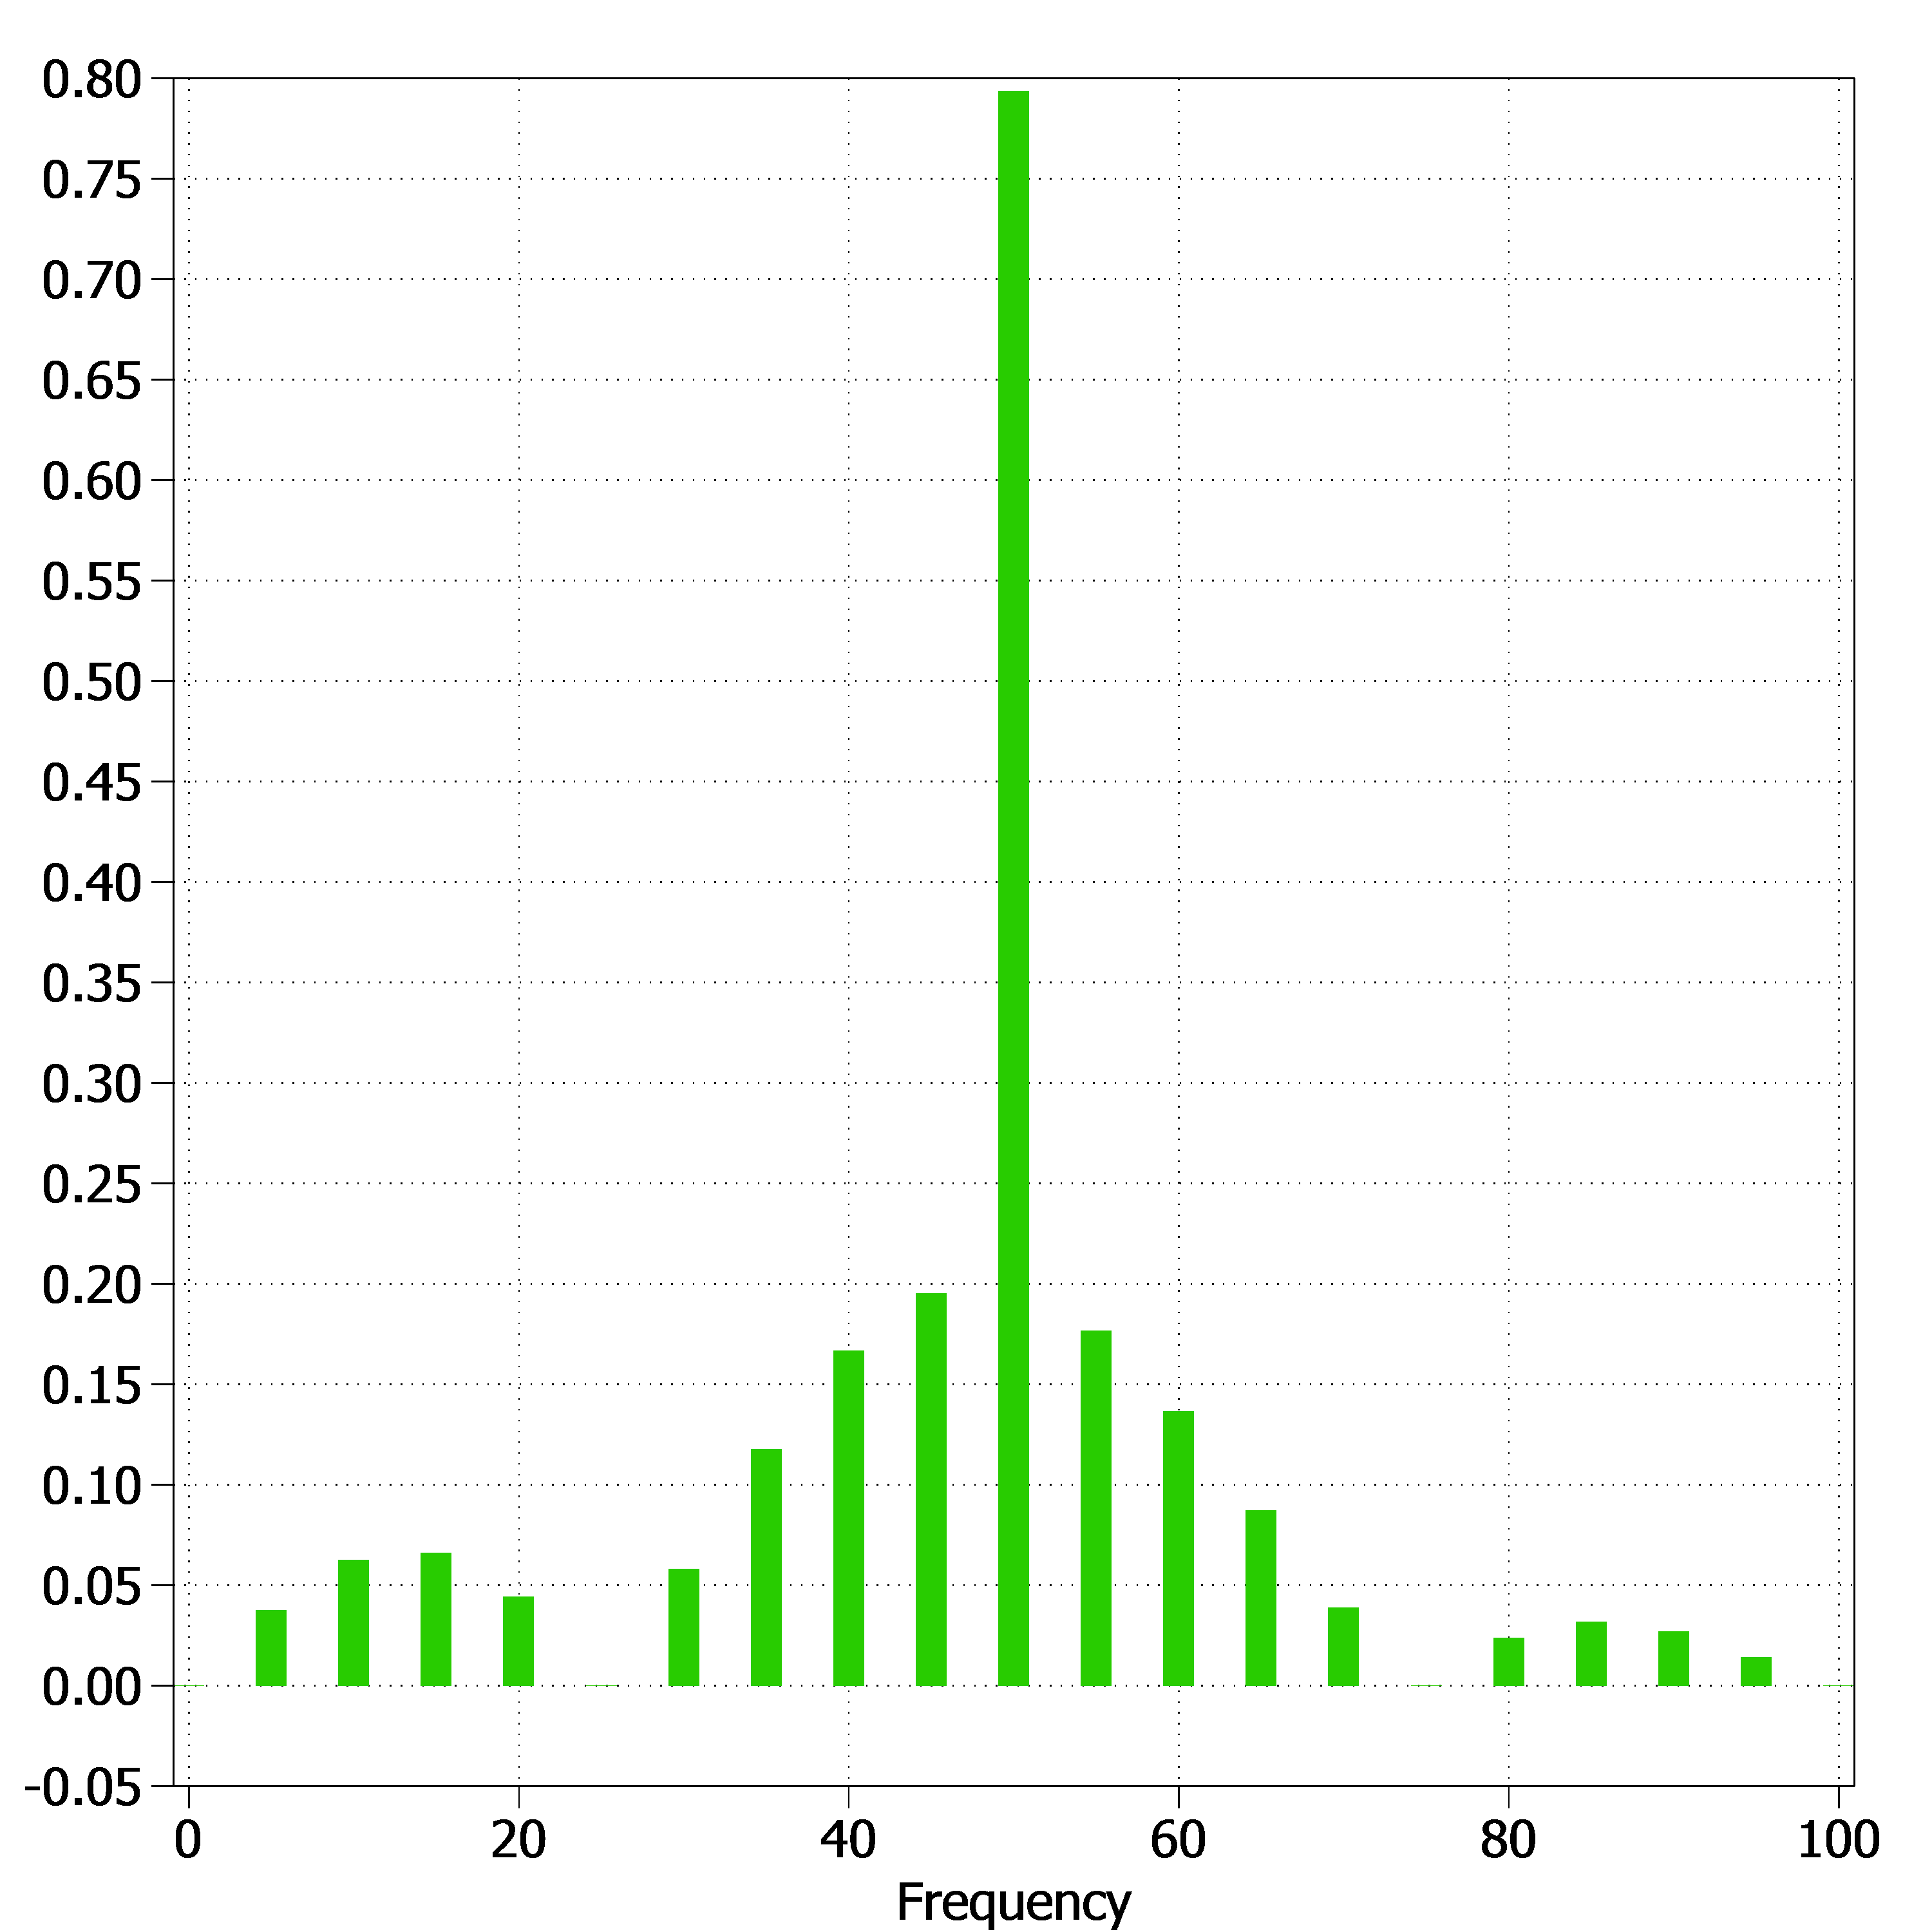
\includegraphics[width=0.45\linewidth]{plecs_schwingungspacket_0_8.PNG}\label{fig:plecs_Schwingungspaket_0_8_100}}\qquad
	\subfloat[][]{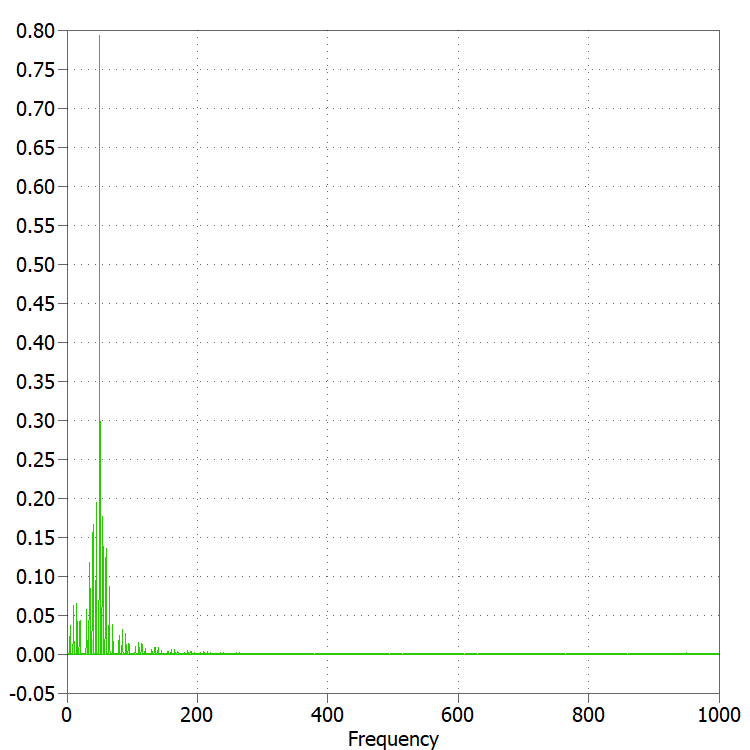
\includegraphics[width=0.45\linewidth]{plecs_schwingungspacket_0_8_1000.PNG}\label{fig:plecs_Schwingungspaket_0_8_1000}}
	\caption{Amplitudenspektrum mit einem duty cycle 0.8 von (a) 0 - 100 Hz (b) 0 - 1000 Hz}
	\label{fig:plecs_Schwingungspakete_Amplitudenspektrum_ 0_8_100_1000}
\end{figure}


Letztlich wurde noch das lineare absolute Spektrum mit den beiden duty cycle 0.5\ref{fig:plecs_Schwingungspaket_0_5_absolut_log} und 0.8\ref{fig:plecs_Schwingungspaket_0_8_absolut_log} veranschaulicht. Damit man die Grafiken mit der Matlab-Simulation vergleichen konnte, entschied man sich das Spektrum nur bis zu einer Frequenz von 100 Hz anzuzeigen. Auch hier erkennt man eine Ähnlichkeit zur Matlab-Simulation. 


\begin{figure}[ht!]
	\centering
	\subfloat[][]{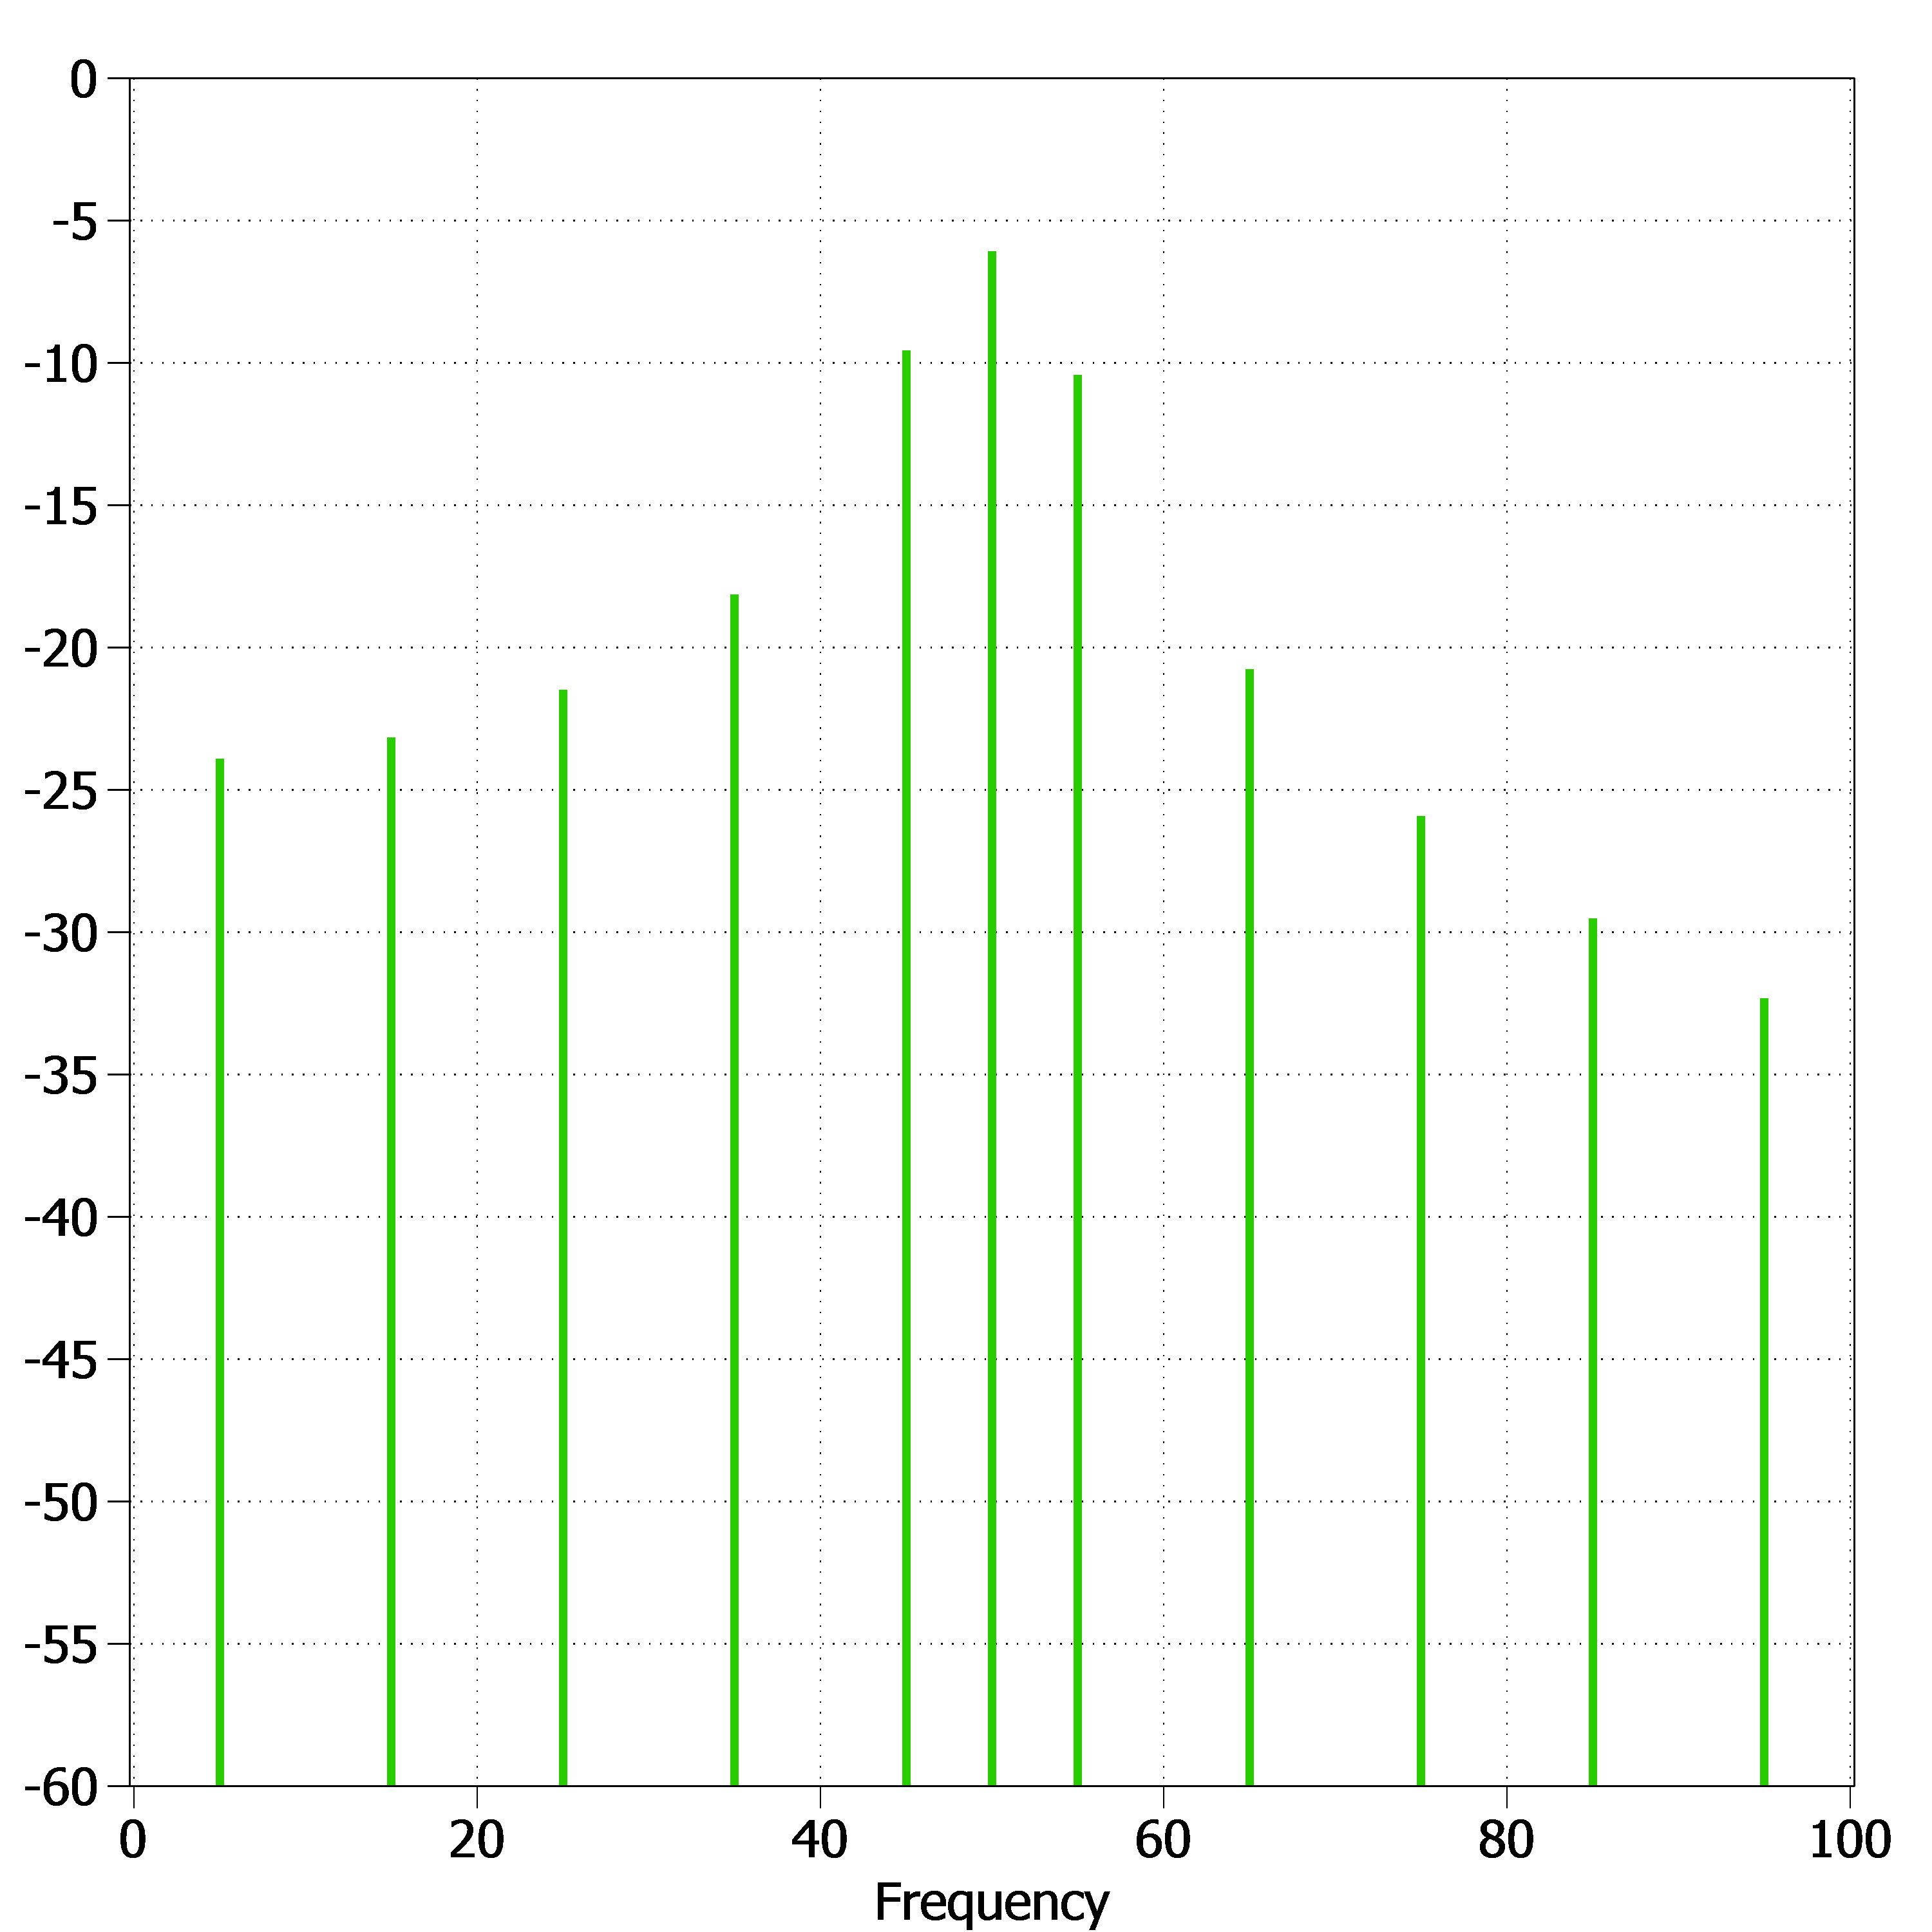
\includegraphics[width=0.45\linewidth]{plecs_schwingungspacket_0_5_absolut_log.PNG}\label{fig:plecs_Schwingungspaket_0_5_absolut_log}}\qquad
	\subfloat[][]{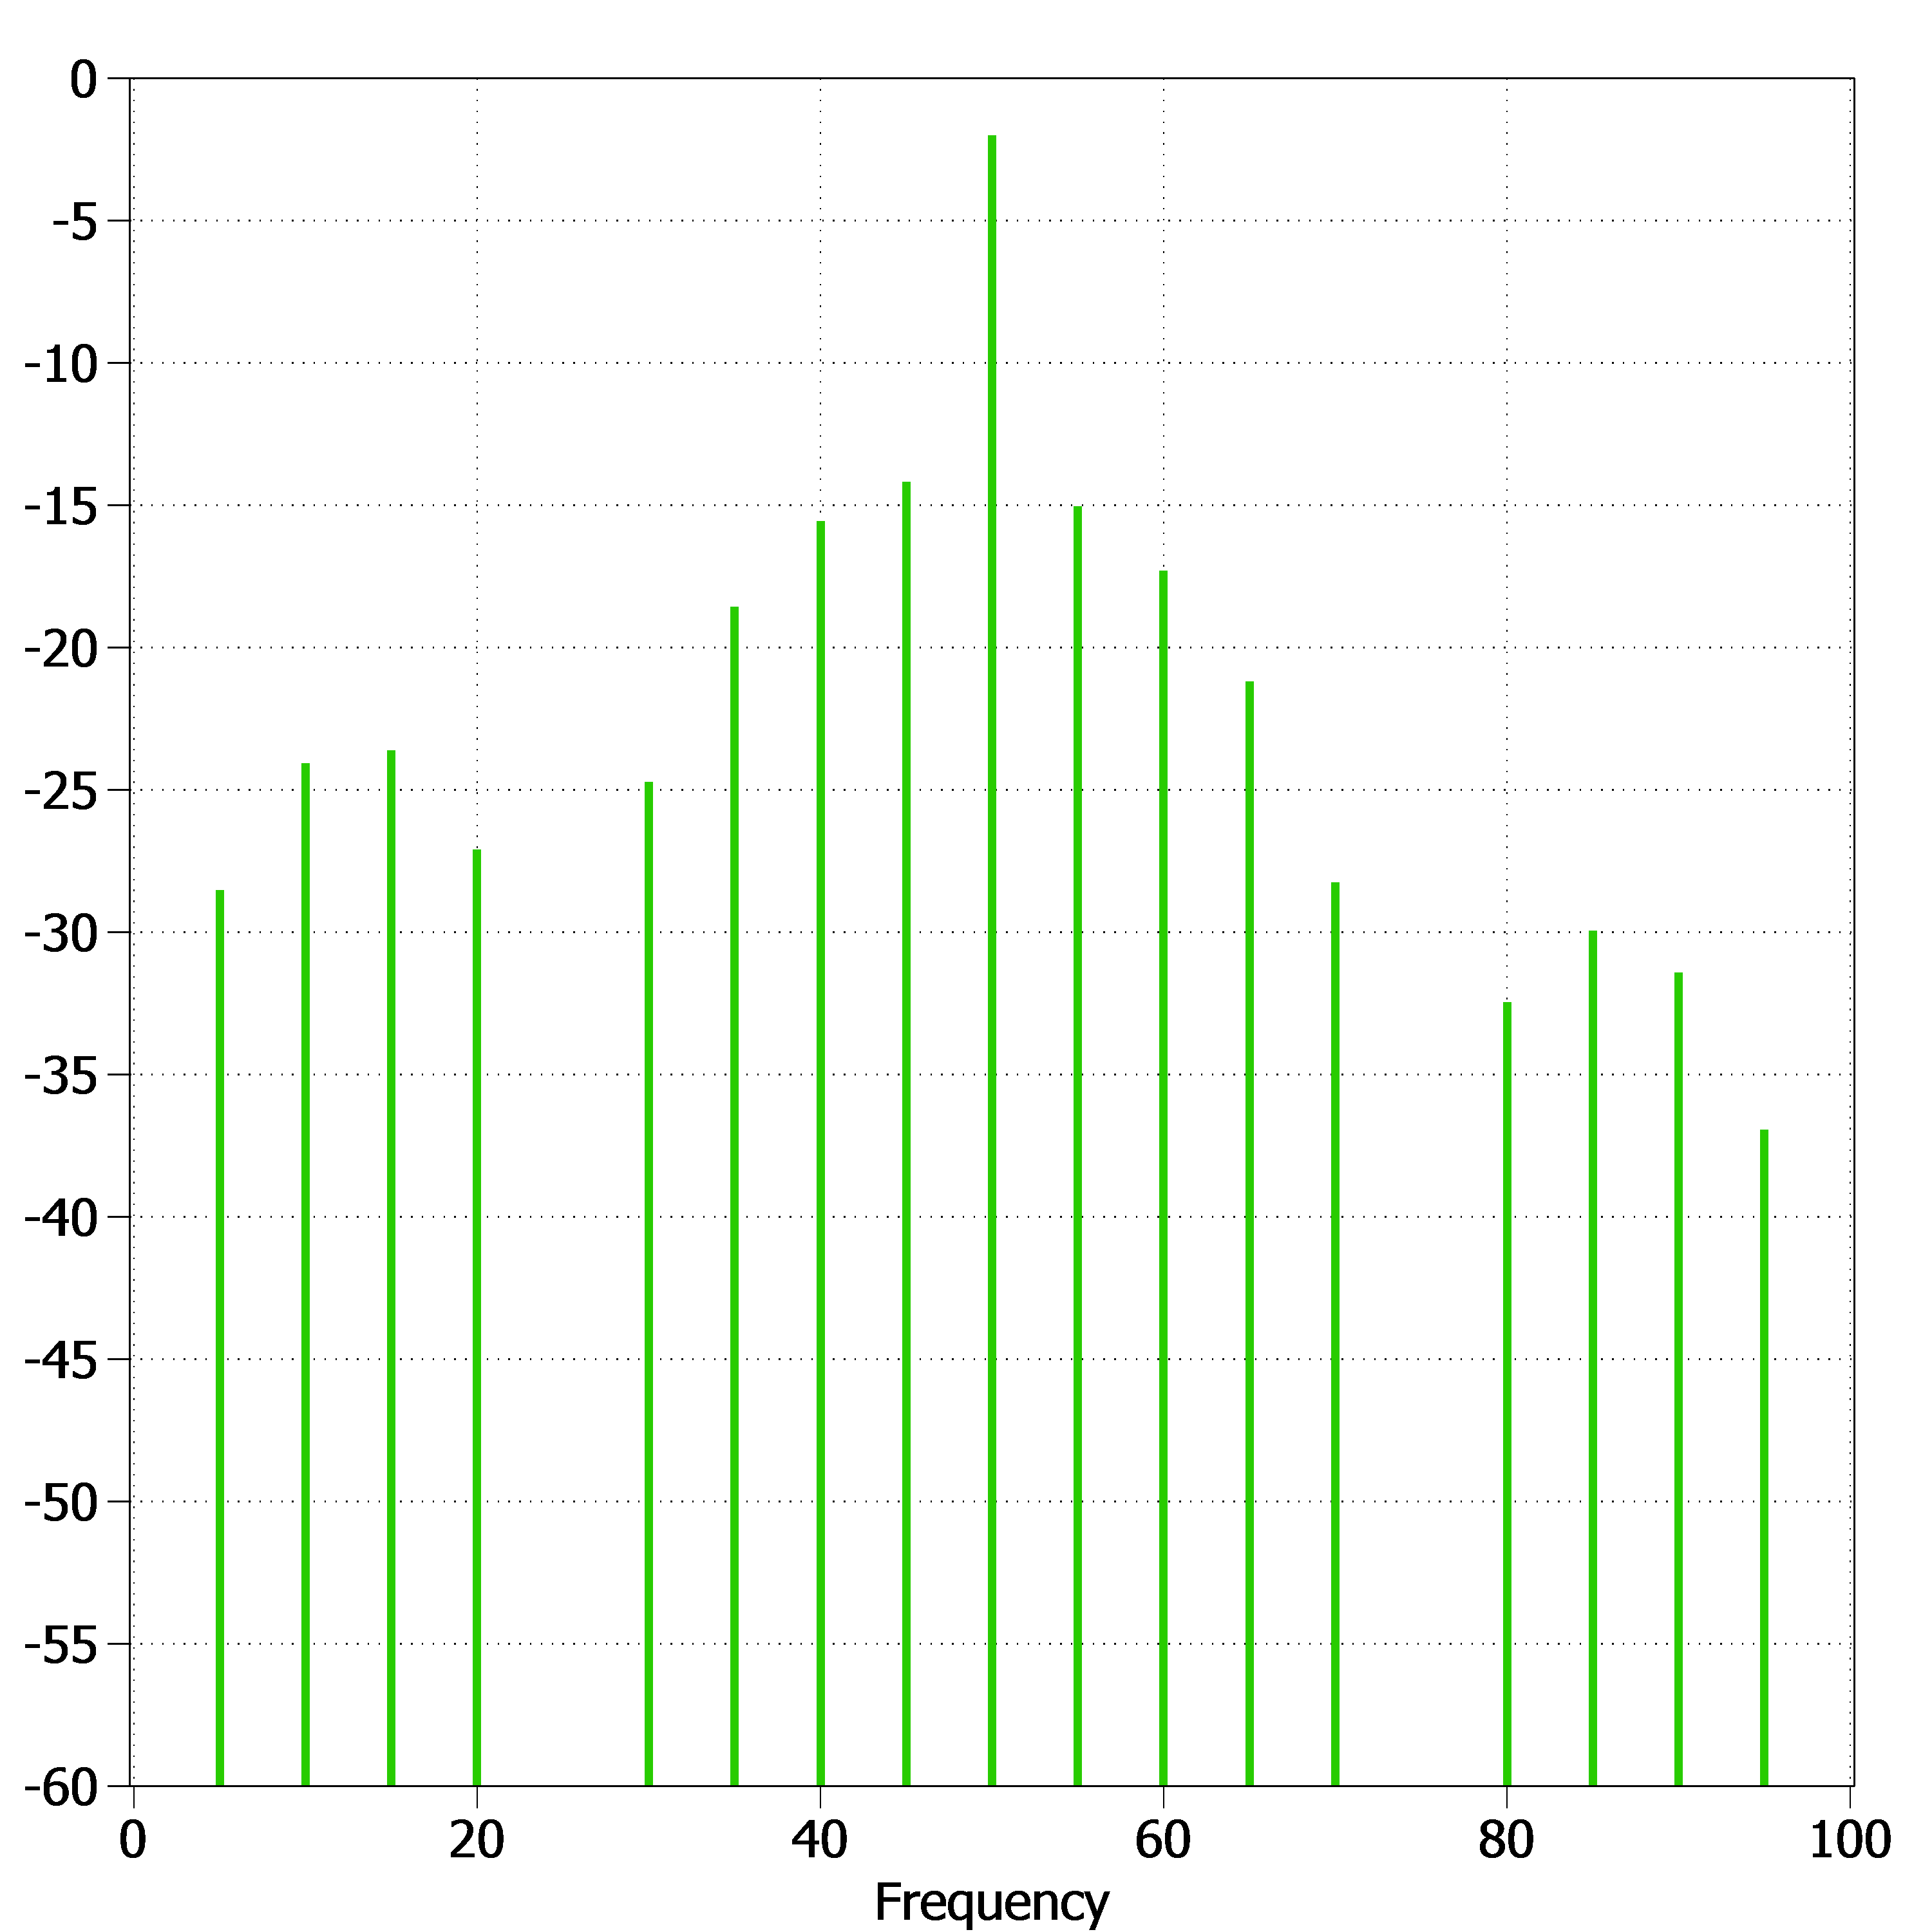
\includegraphics[width=0.45\linewidth]{plecs_schwingungspacket_0_8_absolut_log.PNG}\label{fig:plecs_Schwingungspaket_0_8_absolut_log}}
	\caption{Lineares absolutes Spektrum mit einem duty cycle von (a) 0.5 (b) 0.8}
	\label{fig:plecs_Schwingungspakete_absolut log}
\end{figure}

\subsubsection{Alternative Ansteuerungen}
In der Praxis werden nicht immer alle 3 Phasen angesteuert, sogenannte Sparansteuerungen. Dabei können nur zwei oder auch nur eine Phase angesteuert werden. Das heisst, dass zum Beispiel bei der Zwei-Phasen-Ansteuerung bei einer Phase der Thyristor überbrückt wird beziehungsweise der Thyristor gar nicht vorhanden ist. Dabei dient die überbrückte Phase als Ausgleichs- und Rückleiter. Diese Fälle wurden mit Plecs simuliert wobei die Last in Stern und in Dreieck geschaltet werden kann. Wie bei der 3-Phasen Ansteuerung, wurde für die alternativen Ansteuerung auch der Sanft-Anlass, die Kombination mit Phasenanschnitts- und Schwingungspaketsteuerung, simuliert.

\subsubsection*{2-Phasen Ansteuerung mit Last in Stern}
\todo{Bild Simulation}

 
\subsubsection*{2-Phasen Ansteuerung mit Last in Dreieck}
\todo{Bild Simulation}


\subsubsection*{1-Phasen Ansteuerung mit Last in Stern}
\todo{Bild Simulation}


\subsubsection*{1-Phasen Ansteuerung mit Last in Dreieck}
\todo{Bild Simulation}


\subsubsection*{Halbwellensteuerung}
Eine weitere Möglichkeit, die Thyristoren anzusteuern, ist die Halbwellensteuerung. Dabei wird die positive Halbwelle einer Phasen und zwei negative Halbwellen der anderen Phasen auf die Last geführt. Dies ist mit dem Thyristorsteller, welcher für das Projekt benutzt wurde nicht möglich, da dieser alle 3 Phasen gleich ansteuert. Deshalb wurde dieser Fall nur mit Plecs simuliert. \todo{Einfügen Bild Simulation} Das Problem bei dieser Steuerung ist, dass wenn der Sternpunkt nicht mit dem Nullpunkt verbunden ist, der Phasenverlauf im Plecs schwer zu kontrollieren ist. Da die Summe der Spannungen immer 0 geben muss und die Spannungen phasenverschoben sind gibt es einen sehr unschönen Spannungsverlauf. Wenn das FFT analysiert wird, fällt schnell auf, das die Grundschwingung von 50 Hz nicht den höchsten Peak hat.



